% !TEX program = xelatex
\documentclass[12pt,a4paper]{article}
\setcounter{tocdepth}{3}
\setcounter{secnumdepth}{3}
\usepackage{caption}
\captionsetup[table]{position=bottom}
\captionsetup[figure]{position=bottom}
\usepackage{float}
\usepackage{fontspec}
\setmainfont{Times New Roman}
\renewcommand{\figurename}{Hình}
\renewcommand{\tablename}{Bảng}
\renewcommand{\refname}{TÀI LIỆU THAM KHẢO}
\usepackage{tocloft,calc}
\usepackage[top=3.5cm, bottom=3.0cm, left=3.5cm, right=2.0cm]{geometry} % căn lề theo quy chuẩn KLTN
\usepackage{amsmath,latexsym,amscd,amsfonts,mathrsfs,enumerate} \usepackage{ upgreek }
\usepackage[thref,thmmarks,standard,amsmath,hyperref]{ntheorem}
\usepackage[mathscr]{eucal}
\usepackage[unicode,colorlinks=true, bookmarks=true, pdfstartview=FitH,]{hyperref} %pagebackref=true,
\hypersetup{
pdftitle={Tối ưu hóa đa mục tiêu quy trình lấy hàng trong kho hàng},
pdfauthor={Đặng Anh Tuyền; Phạm Văn Sự},
colorlinks = true,
linkcolor = black,
citecolor = blue,
urlcolor = blue,
}
\usepackage{fancyhdr}
\usepackage{graphicx}
\usepackage{fancybox,cite}
\usepackage{subcaption}
%\usepackage{refcheck}
 
\allowdisplaybreaks
%Môi trường định nghĩa
\theoremheaderfont{\bfseries} % In ra chữ "định nghĩa": đậm, thẳng đứng.
\theorembodyfont{} % Nội dung của định nghia được viết bằng chữ thẳng đứng.
\theoremseparator {}         % Ngăn cách giữa định nghĩa và nội dung định nghĩa bởi dấu chấm.
\newtheorem{dn}{Định nghĩa}[section] % Lệnh này để trong file kết quả in ra chữ nhận xét thay vì nếu ta để mặc định.

%Môi trường Ví dụ
\theoremheaderfont{\bfseries} % In ra chữ "Ví dụ": đậm, thẳng đứng.
\theorembodyfont{\normalfont} % Nội dung của ví dụ được viết bằng chữ thẳng đứng.
\theoremseparator {.}         % Ngăn cách giữa Ví dụ và nội dung ví dụ bởi dấu chấm.
\newtheorem{vd}{Ví dụ}[section] % Lệnh này để trong file kết quả in ra chữ Ví dụ thay vì Example nếu ta để mặc định.

%Môi trường Chú ý
\theoremstyle{plain} %Không đánh sỗ chú ý
\theoremheaderfont{\bfseries} % In ra chữ "chú ý": đậm, thẳng đứng.
\theorembodyfont{\normalfont} % Nội dung của chú ý được viết bằng chữ thẳng đứng.
\theoremseparator {}         % Ngăn cách giữa "chú ý" và nội dung chú ý bởi dấu chấm.
\newtheorem{cy}{Chú ý} % Lệnh này để trong file kết quả in ra chữ "chú ý" thay vì remark nếu ta để mặc định.
\usepackage{booktabs}
\usepackage{longtable}
\usepackage{fvextra}
\usepackage{enumitem}
\setlist{itemsep=3pt,topsep=5pt,parsep=0pt}
\usepackage{tabularx}
\usepackage{multirow}
\usepackage{makecell}
\usepackage{tikz}
\usepackage{xurl}

\Urlmuskip=0mu plus 1mu
\emergencystretch=3em
\usetikzlibrary{arrows.meta,positioning,calc}

% Kiểu dùng chung cho các sơ đồ vector ở Chương 3.
\tikzset{
    chthreeflow/.style={-{Latex[length=2.5mm,width=1.7mm]}, line width=0.9pt, draw=blue!35!black, shorten <=2pt, shorten >=2pt},
    chthreedash/.style={-{Latex[length=2.3mm,width=1.5mm]}, line width=0.85pt, dashed, draw=blue!55!black, shorten <=2pt, shorten >=2pt},
    chthreeblue/.style={draw=blue!70!black, fill=blue!4, rounded corners=5pt, line width=0.8pt, align=center, inner sep=6pt},
    chthreegreen/.style={draw=green!55!black, fill=green!5, rounded corners=5pt, line width=0.8pt, align=center, inner sep=6pt},
    chthreepurple/.style={draw=violet!70!black, fill=violet!5, rounded corners=5pt, line width=0.8pt, align=center, inner sep=6pt},
    chthreeorange/.style={draw=orange!80!black, fill=orange!6, rounded corners=5pt, line width=0.8pt, align=center, inner sep=6pt}
}

% Hiển thị các số phương trình được dẫn lại bằng màu xanh.
\renewcommand{\eqref}[1]{%
    \hyperref[#1]{\textcolor{blue}{\textup{(\ref*{#1})}}}%
}

% Hiển thị số hình được dẫn lại bằng màu xanh, giữ chữ "Hình" màu đen.
\newcommand{\figref}[1]{%
    Hình~\hyperref[#1]{\textcolor{blue}{\ref*{#1}}}%
}

% Hiển thị số bảng được dẫn lại bằng màu xanh, giữ chữ "Bảng" màu đen.
\newcommand{\tabref}[1]{%
    Bảng~\hyperref[#1]{\textcolor{blue}{\ref*{#1}}}%
}

%Môi trường Bài tập
\theoremheaderfont{\bfseries} % In ra chữ "chú ý": đậm, thẳng đứng.
\theorembodyfont{\normalfont} % Nội dung của chú ý được viết bằng chữ thẳng đứng.
\theoremseparator {}         % Ngăn cách giữa "chú ý" và nội dung chú ý bởi dấu chấm.\newtheorem{bt}{Bài tập} % Lệnh này để trong file kết quả in ra chữ "chú ý" thay vì  remark nếu ta để mặc định.

%Môi trường nhân xét
\theoremheaderfont{\bfseries} % In ra chữ "Nhân xét": đậm, thẳng đứng.
\theorembodyfont{\normalfont} % Nội dung của nhạn xét được viết bằng chữ thẳng đứng.
\theoremseparator {}         % Ngăn cách giữa nhận xét và nội dung nhận xét bởi dấu chấm.
\newtheorem{nx}{Nhận xét}[section] % Lệnh này để trong file kết quả in ra chữ nhận xét thay vì nếu ta để mặc định.

%Môi trường định lý
\theoremstyle{plain} %Sử dụng phong cách plain để đánh số Định lý, chẳng hạn: Định lý 1, Định lý 2,...
\theoremheaderfont{\normalfont\bfseries} % In ra chữ "Định lý": đậm, thẳng đứng.
\theorembodyfont{\normalfont} % Nội dung của Định lý được viết bằng chữ nghiêng.
\theoremseparator {.}         % Ngăn cách giữa Định lý và nội dung định lý bởi dấu chấm.
\renewtheorem{theorem}{Định lý} % Lệnh này để trong file kết quả in ra chữ Định lý thay vì theorem nếu ta để mặc định.
%Môi trường Mệnh đề
\theoremstyle{plain} %Sử dụng phong cách plain để đánh số Mệnh đề, chẳng hạn: Mệnh đề 1, Mệnh đề 2,...
\theoremheaderfont{\normalfont\bfseries} % In ra chữ "Mệnh đề": đậm, thẳng đứng.
\theorembodyfont{\normalfont} % Nội dung của Mệnh đề được viết bằng chữ thẳng đứng.
\theoremseparator {.}         % Ngăn cách giữa Mệnh đề và nội dung mệnh đề bởi dấu chấm.
\renewtheorem{proposition}{Mệnh đề} % Lệnh này để trong file kết quả in ra chữ Mệnh đề thay vì proposition nếu ta để mặc định.
%Môi trường Chứng minh
\theoremstyle{nonumberplain}  % Kiểu định dạng dành cho chứng minh
\theoremheaderfont{\normalfont\bfseries} % Tiêu đề "Chứng minh" in nghiêng
\theorembodyfont{\normalfont}
\theoremseparator{.} 
\theoremsymbol{\ensuremath{\square}} % Dấu kết thúc chứng minh là ô vuông
\newtheorem{cm}{Chứng minh}[section]

\pagestyle{fancy}
\fancyhf{}
\fancyhead[L]{\itshape Thuật toán ứng dụng}
\fancyfoot[L]{\fontsize{9}{11}\selectfont\itshape Tối ưu hóa đa mục tiêu quy trình lấy hàng trong kho hàng}
\fancyfoot[R]{\fontsize{9}{11}\selectfont\thepage}
\setlength{\headheight}{16pt}
\renewcommand{\headrulewidth}{1.2pt}
\renewcommand{\footrulewidth}{1.2pt} % Tiêu đề chân trang
\fancypagestyle{plain}{
    \fancyhf{}
    \fancyhead[L]{\itshape Thuật toán ứng dụng}
    \fancyfoot[L]{\fontsize{9}{11}\selectfont\itshape Tối ưu hóa đa mục tiêu quy trình lấy hàng trong kho hàng}
    \fancyfoot[R]{\fontsize{9}{11}\selectfont\thepage}
    \renewcommand{\headrulewidth}{1.2pt}
    \renewcommand{\footrulewidth}{1.2pt}
}

\numberwithin{equation}{section}
\numberwithin{figure}{section}
\numberwithin{table}{section}

\begin{document}
\newcommand{\mapsBzero}{25,33}
\newcommand{\mapsBtwo}{13,40}
\newcommand{\mapsLNS}{-0,02}
\newcommand{\mapsVNS}{-2,02}
\newcommand{\scalabilityBzero}{27,40}
\newcommand{\scalabilityBtwo}{6,58}
\newcommand{\scalabilityLNS}{0,14}
\newcommand{\scalabilityVNS}{-2,25}
\newcommand{\krisBzero}{17,68}
\newcommand{\krisBtwo}{9,18}
\newcommand{\krisLNS}{0,07}
\newcommand{\krisVNS}{0,01}

 \fontsize{13pt}{18pt}\selectfont
 \hypersetup{pageanchor=false}
 
 \thisfancypage{\setlength{\fboxsep}{0.2cm}\setlength{\fboxrule}{1pt}\doublebox}{}
 \begin{titlepage}
\begin{center}
	\large
	BỘ GIÁO DỤC VÀ ĐÀO TẠO\\
	\textbf{ĐẠI HỌC PHENIKAA}\\
	\textbf{TRƯỜNG CÔNG NGHỆ THÔNG TIN}\\[0.15cm]
	\rule{3.2cm}{0.4pt}\,o0o\,\rule{3.2cm}{0.4pt}
\end{center}
\vspace{-0.5cm}
\begin{center}
    
\includegraphics[scale=0.8]{image/Logo.png}\\[1cm] 
\end{center} 
\vspace{0.3 cm}
\begin{center}
    \bf\Large {BÁO CÁO BÀI TẬP LỚN}
\end{center}
\begin{center}
    \bf\large {HỌC PHẦN: THUẬT TOÁN ỨNG DỤNG}
\end{center}
\vspace{0.3 cm}
\begin{center}
	\bf\large ĐỀ TÀI: TỐI ƯU HÓA ĐA MỤC TIÊU QUY TRÌNH LẤY HÀNG TRONG KHO HÀNG
\end{center}
\begin{center}
	\normalsize
	\renewcommand{\arraystretch}{1.15}
	\begin{tabular}{@{}p{5.2cm}l@{}}
        \textbf{Đặng Anh Tuyền} & \textbf{MSSV:} 23010912 \\
                                & \textbf{Lớp:} K17-KHMT(AI\&KHDL)\_1 \\[0.25cm]
        \textbf{Phạm Văn Sự} & \textbf{MSSV:} 23010523 \\
                                & \textbf{Lớp:} K17-KHMT(AI\&KHDL)\_1
	\end{tabular}
\end{center}

\vskip 0.8 cm
  \begin{center}
   GVHD: TS. Trần Đình Tân
  \end{center}
\vskip 0.5 cm
  \begin{center}
   {\large\textbf{Hà Nội, Năm 2026}}
  \end{center}
 \end{titlepage}

% Bìa lót: bố cục học thuật theo mẫu, có khung đôi và không sử dụng logo.
\begin{titlepage}
\thispagestyle{empty}
\thisfancypage{\setlength{\fboxsep}{0.2cm}\setlength{\fboxrule}{1pt}\doublebox}{}
\begin{center}
	\large
	BỘ GIÁO DỤC VÀ ĐÀO TẠO\\
	\textbf{ĐẠI HỌC PHENIKAA}\\
	\textbf{TRƯỜNG CÔNG NGHỆ THÔNG TIN}\\[0.15cm]
	\rule{4cm}{0.4pt}\,o0o\,\rule{4cm}{0.4pt}
\end{center}
\vspace{1.5cm}
\begin{center}
	\normalsize
	\renewcommand{\arraystretch}{1.15}
	\begin{tabular}{@{}p{5.2cm}l@{}}
        \textbf{Đặng Anh Tuyền} & \textbf{MSSV:} 23010912 \\
                                & \textbf{Lớp:} K17-KHMT(AI\&KHDL)\_1 \\[0.25cm]
        \textbf{Phạm Văn Sự} & \textbf{MSSV:} 23010523 \\
                                & \textbf{Lớp:} K17-KHMT(AI\&KHDL)\_1
	\end{tabular}
\end{center}
\vspace{1.3cm}
\begin{center}
    \bf\Large {BÁO CÁO BÀI TẬP LỚN}
\end{center}
\begin{center}
    \bf\large {HỌC PHẦN: THUẬT TOÁN ỨNG DỤNG}
\end{center}
\vspace{0.65cm}
\begin{center}
	\bf\Large TỐI ƯU HÓA ĐỒNG THỜI GOM ĐƠN, ĐỊNH TUYẾN\\
    VÀ LẬP LỊCH TRONG KHO HÀNG
\end{center}
\vfill
\begin{center}
    GVHD: TS. Trần Đình Tân
\end{center}
\vfill
\begin{center}
    {\large\textbf{Hà Nội, Năm 2026}}
\end{center}
\vspace{0.25cm}
\end{titlepage}

% Bảng phân chia công việc của nhóm.
\begin{titlepage}
\thispagestyle{empty}
\begin{center}
    {\bfseries\Large BẢNG PHÂN CHIA CÔNG VIỆC}
\end{center}
\vspace{0.45cm}

\begingroup
\fontsize{10.5pt}{12.5pt}\selectfont
\setlength{\tabcolsep}{3.5pt}
\setlength{\arrayrulewidth}{0.7pt}
\renewcommand{\arraystretch}{1.08}
\begin{center}
\begin{tabularx}{\textwidth}{|
    >{\centering\arraybackslash}m{0.8cm}|
    >{\centering\arraybackslash}m{3.5cm}|
    >{\centering\arraybackslash}m{1.75cm}|
    >{\raggedright\arraybackslash}X|
    >{\centering\arraybackslash}m{1.45cm}|}
\hline
\textbf{STT} & \centering\textbf{Họ và tên} & \textbf{Vai trò} & \centering\textbf{Nội dung công việc} & \textbf{Tỷ lệ} \\
\hline
1 & \makecell[c]{Đặng Anh Tuyền} & \textbf{Trưởng nhóm} &
-- Lập kế hoạch, phân công và theo dõi tiến độ chung.\newline
-- Thiết kế mô hình toán học và cấu trúc dữ liệu đồ thị kho hàng.\newline
-- Cài đặt thuật toán ALNS (Adaptive Large Neighborhood Search).\newline
-- Xây dựng hệ thống sinh dữ liệu 5 kịch bản kho và benchmark đối chuẩn.\newline
-- Phát triển giao diện Web Streamlit và mô phỏng Canvas.\newline
-- Hoàn thiện báo cáo và slide thuyết trình. & \textbf{50\%} \\
\hline
2 & \makecell[c]{Phạm Văn Sự} & Thành viên &
-- Tìm hiểu cơ sở lý thuyết gom đơn, định tuyến và lập lịch (JOBPRSP).\newline
-- Cài đặt và cấu hình các thuật toán cơ sở B0, B1, B2, B3 và VNS/LNS.\newline
-- Thực hiện thử nghiệm và thu thập số liệu đối chuẩn bộ dữ liệu Kris.\newline
-- Vẽ biểu đồ so sánh, phân tích kết quả thực nghiệm và kiểm định nghiệm.\newline
-- Rà soát nội dung, chính tả và chuẩn hóa báo cáo LaTeX.\newline
-- Chuẩn bị slide và thuyết trình. & \textbf{50\%} \\
\hline
\end{tabularx}
\end{center}
\endgroup

\vspace{0.55cm}
\begin{center}
    {\fontsize{13pt}{16pt}\selectfont
    \textbf{Repository dự án:}\quad
    \href{https://github.com/tuyenda2011/TTUD_v2}{\texttt{github.com/tuyenda2011/TTUD\_v2}}}
\end{center}
\end{titlepage}

\pagestyle{fancy}
\pagenumbering{arabic}
\setcounter{page}{1}
\hypersetup{pageanchor=true,linkcolor=black}

\section*{DANH MỤC TỪ VIẾT TẮT}
\addcontentsline{toc}{section}{DANH MỤC TỪ VIẾT TẮT}
\begin{tabularx}{\linewidth}{lX}
\toprule
Ký hiệu & Ý nghĩa \\
\midrule
JOBPRSP & Bài toán tích hợp gom đơn, định tuyến và lập lịch nhân viên lấy hàng. \\
ALNS & Adaptive Large Neighborhood Search: tìm kiếm lân cận lớn thích ứng. \\
LNS & Large Neighborhood Search: tìm kiếm lân cận lớn. \\
VNS & Variable Neighborhood Search: tìm kiếm biến đổi lân cận. \\
SA & Simulated Annealing: luyện kim mô phỏng. \\
NN & Nearest Neighbor: láng giềng gần nhất. \\
EDD & Earliest Due Date: ưu tiên hạn hoàn thành sớm nhất. \\
FCFS & First Come, First Served: phục vụ theo thứ tự đến. \\
SKU & Stock Keeping Unit: mã phân biệt sản phẩm lưu kho. \\
\bottomrule
\end{tabularx}
\clearpage

% Chèn mục lục
\renewcommand{\contentsname}{Mục lục}
\tableofcontents

% Ngắt trang tại đây để chuyển Danh mục hình ảnh sang trang mới
\newpage 
%\clearpage % (Bạn cũng có thể dùng \clearpage thay cho \newpage)

% Chèn danh mục hình ảnh
\renewcommand{\listfigurename}{Danh sách hình ảnh}
\listoffigures

% Chèn danh mục bảng
\clearpage
\renewcommand{\listtablename}{Danh sách bảng}
\listoftables

% Ngắt trang để phần nội dung bài viết bắt đầu ở trang mới
\clearpage
\section{TỔNG QUAN ĐỀ TÀI}
\label{sec:chuong1}

\subsection{Bối cảnh và nhu cầu tối ưu quy trình lấy hàng trong kho}
Lấy hàng là quá trình thu gom sản phẩm tại các vị trí lưu trữ để đáp ứng yêu cầu của đơn hàng. Nhân viên di chuyển từ điểm tập kết đến các vị trí cần lấy, thu gom sản phẩm và quay về điểm tập kết khi kết thúc chuyến. Trong báo cáo, điểm tập kết được gọi là depot; một mã hàng phân biệt sản phẩm được gọi là Stock Keeping Unit (SKU). Một đơn có thể gồm nhiều mã hàng nằm ở các vị trí khác nhau, còn một chuyến có thể phục vụ nhiều đơn nếu tổng tải không vượt sức chứa xe đẩy.

Khi nhiều đơn cùng chờ xử lý, cách tổ chức lấy hàng ảnh hưởng đến cả quãng đường di chuyển và thời điểm hoàn thành. Phục vụ từng đơn riêng lẻ có thể làm nhân viên đi lặp lại các đoạn đường. Gom đơn cho phép chia sẻ lộ trình, nhưng cũng có thể kéo dài chuyến và khiến đơn có hạn gần phải chờ lâu hơn. Khi có nhiều nhân viên, việc phân công và sắp xếp chuyến còn quyết định mức cân bằng công việc giữa các nhân viên.

Tổng quan của de Koster và cộng sự \cite{dekoster2007} hệ thống hóa các quyết định về thiết kế và điều hành hoạt động lấy hàng, trong đó có định tuyến và gom đơn. Với mô hình được xét trong đề tài, yêu cầu đặt ra là xây dựng kế hoạch phục vụ đủ đơn, tuân thủ sức chứa và các lối đi của kho, đồng thời cân đối quãng đường, thời gian hoàn tất và trễ hạn. Đây là cơ sở để lựa chọn một bài toán tối ưu có sự kết hợp giữa nhiều quyết định vận hành.

\subsection{Bài toán tích hợp gom đơn, định tuyến và lập lịch}
Đề tài xét bài toán tích hợp ba quyết định: gom đơn xác định các đơn được phục vụ trong cùng một chuyến; định tuyến xác định thứ tự ghé các vị trí lấy hàng và đường đi giữa chúng; lập lịch xác định nhân viên phụ trách cùng thứ tự thực hiện các chuyến của mỗi người. Một nghiệm hoàn chỉnh phải thể hiện được cả ba quyết định này.

Các quyết định có quan hệ chặt chẽ. Thêm một đơn vào chuyến làm thay đổi tập vị trí cần ghé và có thể làm tăng thời lượng chuyến. Các chuyến tiếp theo của cùng nhân viên khi đó phải bắt đầu muộn hơn, ảnh hưởng đến thời điểm hoàn thành những đơn khác. Ngược lại, thay đổi nhân viên phụ trách hoặc thứ tự chuyến có thể giảm trễ mà không cần thay đổi cách gom đơn.

Chẳng hạn, hai đơn có sản phẩm gần nhau nhưng hạn hoàn thành khác nhau có thể được gom để chia sẻ lộ trình. Tuy nhiên, trong mô hình của đề tài, đơn chỉ hoàn thành khi chuyến chứa nó quay về depot; vì vậy đơn gấp có thể phải chờ việc lấy hàng của đơn còn lại. Tách đơn gấp thành chuyến riêng có thể giảm trễ nhưng làm tăng quãng đường. Ví dụ này cho thấy một thay đổi có lợi cho một chỉ tiêu chưa chắc có lợi cho các chỉ tiêu còn lại.

Đề tài sử dụng hạn hoàn thành mềm: một đơn được phép hoàn thành sau hạn, nhưng phần thời gian vượt hạn được tính vào chi phí. Chất lượng nghiệm được đánh giá bằng tổng có trọng số của ba thành phần đã chuẩn hóa: tổng quãng đường, thời gian hoàn tất toàn bộ công việc (makespan) và tổng độ trễ. Số đơn trễ được theo dõi như một chỉ tiêu bổ sung. Khi phân tích thực nghiệm, cần xem cả mục tiêu tổng hợp lẫn từng thành phần để nhận diện các đánh đổi.

\subsection{Các hướng giải quyết liên quan}
Các nghiên cứu về lấy hàng có thể tập trung vào một quyết định riêng hoặc xét nhiều quyết định đồng thời. Gademann và van de Velde \cite{gademann2005} nghiên cứu gom đơn nhằm giảm tổng thời gian di chuyển trong kho có các lối song song. Ratliff và Rosenthal \cite{ratliff1983} xây dựng phương pháp định tuyến cho một trường hợp kho chữ nhật với lối nối ở hai đầu dãy. Hai công trình cung cấp cơ sở tham khảo cho việc tổ chức nhóm đơn và khai thác cấu trúc đường đi.

Ở hướng tích hợp, Briant và cộng sự \cite{briant2023} xét bài toán gom đơn, định tuyến và sắp thứ tự có hạn hoàn thành, sử dụng mô hình quy hoạch tuyến tính và phương pháp sinh cột để xây dựng cận dưới và cận trên. Đề tài tham khảo cách tiếp cận tích hợp, nhưng sử dụng mô hình có hạn mềm và mục tiêu gồm ba thành phần. Vì khác biệt về mô hình và tiêu chí đánh giá, kết quả được đối chiếu giữa các phương pháp cài đặt trong đề tài trên cùng dữ liệu và cùng bộ đánh giá.

Về tìm kiếm nghiệm, Shaw \cite{shaw1998} trình bày Large Neighborhood Search (LNS), thay đổi một phần nghiệm bằng cách loại bỏ và chèn lại các phần tử. Ropke và Pisinger \cite{ropke2006} phát triển Adaptive Large Neighborhood Search (ALNS), trong đó tần suất sử dụng các toán tử phụ thuộc vào hiệu quả đã quan sát. Mladenović và Hansen \cite{mladenovic1997} đề xuất Variable Neighborhood Search (VNS), dựa trên việc thay đổi có hệ thống cấu trúc lân cận. Các khung này là cơ sở để xây dựng những chiến lược cải thiện nghiệm khác nhau cho bài toán kho hàng.

\begin{table}[H]
\centering\small
\begin{tabularx}{\linewidth}{lXX}
\toprule
Tài liệu & Hướng tiếp cận & Nội dung tham khảo \\
\midrule
de Koster và cộng sự \cite{dekoster2007} & Tổng quan hoạt động lấy hàng. & Các quyết định về gom đơn và định tuyến. \\
Gademann--van de Velde \cite{gademann2005} & Gom đơn theo thời gian di chuyển. & Quan hệ giữa nhóm đơn và chi phí lấy hàng. \\
Ratliff--Rosenthal \cite{ratliff1983} & Định tuyến trong kho chữ nhật. & Khai thác cấu trúc lối đi. \\
Briant và cộng sự \cite{briant2023} & Tối ưu tích hợp có hạn hoàn thành. & Mô hình tích hợp và cách xây dựng cận. \\
Shaw \cite{shaw1998} & LNS. & Loại bỏ và tái chèn một phần nghiệm. \\
Ropke--Pisinger \cite{ropke2006} & ALNS. & Lựa chọn toán tử theo hiệu quả quan sát. \\
Mladenović--Hansen \cite{mladenovic1997} & VNS. & Thay đổi cấu trúc lân cận. \\
\bottomrule
\end{tabularx}
\caption{Các hướng giải quyết liên quan và nội dung tham khảo.}\label{tab:related-work}
\end{table}

Trên cơ sở các hướng trong \tabref{tab:related-work}, đề tài cài đặt năm phương pháp: First-Come, First-Served Batching (B0), Greedy Batching (B2), LNS, ALNS và VNS. B0 là mốc kiến tạo đơn giản, gom đơn theo thứ tự đầu vào; B2 sử dụng tiêu chí tham lam để xây dựng nghiệm và làm điểm xuất phát cho ba phương pháp tìm kiếm. So sánh LNS với ALNS nhằm khảo sát lựa chọn toán tử đều và lựa chọn thích ứng trên cùng bộ toán tử. VNS bổ sung một chiến lược đối chứng dựa trên thay đổi cấu trúc lân cận. Cách lựa chọn này cho phép đánh giá từ nghiệm cơ sở đến các cơ chế cải thiện nghiệm, với cùng mô hình và hàm mục tiêu.

Trong cài đặt, B0 dựng tuyến bằng Nearest Neighbor, còn B2 kết hợp Nearest Neighbor với 2-Opt. Vì vậy, so sánh B2 với B0 phản ánh sự khác biệt của cả cách gom đơn và cách định tuyến; không quy toàn bộ chênh lệch chất lượng nghiệm cho riêng bước gom đơn tham lam. Các đối chiếu với B2 cho biết lợi ích của việc tiếp tục tìm kiếm trong ngân sách đã xét, nhưng không bảo đảm một phương pháp luôn tốt hơn trên mọi đầu vào.

\subsection{Mục tiêu và phạm vi đề tài}
Mục tiêu của đề tài là xây dựng và phân tích các thuật toán giải bài toán tích hợp gom đơn, định tuyến và lập lịch, đồng thời đánh giá chất lượng nghiệm và chi phí tính toán của năm phương pháp. Phần thuật toán trình bày nguyên lý, giả mã, ví dụ minh họa và phân tích chi phí của cài đặt. Phần thực nghiệm đối chiếu kết quả trên các nhóm dữ liệu, liên hệ những khác biệt quan sát được với cơ chế tìm kiếm và điều kiện chạy.

Trong phần thực nghiệm, thời gian tính toán là thời gian chương trình chạy để xây dựng và kiểm chứng kế hoạch. Đại lượng này được phân biệt với makespan, là thời gian hoàn tất công việc theo lịch thực hiện trong mô hình kho. Một thuật toán chạy nhanh trên máy tính chưa chắc tạo ra kế hoạch có makespan thấp, và ngược lại.

Các sản phẩm chính gồm bộ giải cài đặt năm phương pháp trên cùng mô hình và bộ đánh giá; cơ chế kiểm chứng tính hợp lệ của nghiệm cùng các chỉ tiêu được xuất ra; và bộ thực nghiệm lưu cấu hình, đầu vào, nghiệm và số liệu để tổng hợp kết quả so sánh. Giao diện mô phỏng hỗ trợ quan sát tuyến đi và lịch thực hiện. Đóng góp của đề tài tập trung vào việc áp dụng, cài đặt và kiểm chứng các phương pháp trong phạm vi bài toán đã xác định, không khẳng định một khung thuật toán mới.

Các câu hỏi đánh giá chính gồm:
\begin{enumerate}
\item Chất lượng nghiệm của B2 khác B0 như thế nào?
\item Tiếp tục tìm kiếm từ nghiệm B2 làm thay đổi chất lượng nghiệm và thời gian tính toán như thế nào?
\item Với cùng bộ toán tử và ngân sách, lựa chọn thích ứng của ALNS cho kết quả khác LNS như thế nào?
\item Chiến lược thay đổi lân cận của VNS cho chất lượng nghiệm, độ ổn định và thời gian tính toán như thế nào so với LNS và ALNS?
\item Quy mô bài toán và ngân sách tìm kiếm ảnh hưởng thế nào đến chất lượng nghiệm và thứ hạng các phương pháp?
\item Thay đổi trọng số mục tiêu tạo ra những đánh đổi nào giữa quãng đường, thời gian hoàn tất và độ trễ?
\end{enumerate}

Phạm vi nghiên cứu là kho tĩnh với số nhân viên cho trước, nhân viên đồng nhất về tốc độ và thời gian thao tác, cùng xe đẩy có sức chứa hữu hạn. Toàn bộ đơn được biết và sẵn sàng tại thời điểm bắt đầu; mỗi đơn được phục vụ trọn vẹn trong một chuyến và hoàn thành khi chuyến quay về depot. Mô hình chưa xét đơn phát sinh trong quá trình vận hành, ca nghỉ hoặc xung đột di chuyển giữa nhân viên.

Thực nghiệm sử dụng các bản đồ kho tổng hợp, nhóm dữ liệu thay đổi quy mô và bộ dữ liệu tham chiếu Kris Small. Kết quả được tổng hợp riêng theo nhóm dữ liệu; các trường hợp nổi bật được lựa chọn để phân tích cùng với bảng kết quả đầy đủ. Việc đánh giá bao gồm kiểm tra tính hợp lệ của nghiệm, chất lượng mục tiêu, các thành phần vận hành, hội tụ và độ ổn định qua các lần chạy. Các kết luận được giới hạn trong mô hình, dữ liệu và ngân sách đã khảo sát; kết quả trên dữ liệu mô phỏng chưa đủ để khẳng định hiệu quả trong mọi kho thực tế hoặc bảo đảm tối ưu toàn cục.

\clearpage
\section{MÔ HÌNH HÓA BÀI TOÁN}
\label{sec:chuong2}

\subsection{Dữ liệu đầu vào và các giả định}

Một đầu vào xác định kho hàng, tập đơn cần phục vụ và các thông số vận hành. Gọi $O$ là tập đơn, $K$ là tập sản phẩm và $P=\{1,\ldots,m\}$ là tập nhân viên, với $n=|O|>0$. Đơn $i\in O$ yêu cầu số lượng $q_{is}$ của sản phẩm $s$; quy ước $q_{is}=0$ nếu đơn không yêu cầu sản phẩm đó. Mỗi sản phẩm có vị trí lấy hàng $\ell_s$, tải của một đơn vị $a_s>0$ và thời gian lấy một đơn vị $h_s\geq0$. Tải của đơn được tính bởi
\begin{equation}
 w_i=\sum_{s\in K}a_sq_{is}.\label{eq:model-order-load}
\end{equation}
Đơn có hạn hoàn thành $d_i\geq0$ và một thứ tự đầu vào. Thứ tự này phục vụ việc gom đơn cơ sở, không phải thời điểm đơn phát sinh.

Thông số vận hành gồm sức chứa xe $Q>0$, vận tốc di chuyển $v>0$, thời gian chuẩn bị mỗi chuyến $b\geq0$ và thời gian thao tác cố định tại mỗi vị trí có yêu cầu lấy hàng $h_{\rm loc}\geq0$. Sức chứa và tải sản phẩm dùng cùng một đơn vị tải quy ước, không mặc định là khối lượng. Dữ liệu mô phỏng dùng mét và phút; dữ liệu Kris giữ quy ước số học của nguồn. Trong từng đầu vào, khoảng cách, vận tốc và thời gian phải nhất quán. Việc quy đổi đơn vị hiển thị không thay thế việc đánh giá nghiệm theo dữ liệu nguồn.

\begin{table}[H]
\centering\small
\begin{tabularx}{\linewidth}{lX}
\toprule
Ký hiệu & Ý nghĩa \\
\midrule
$O,K,P$ & Tập đơn, tập sản phẩm và tập nhân viên. \\
$n,m$ & Số đơn và số nhân viên. \\
$q_{is},a_s,h_s$ & Số lượng yêu cầu, tải và thời gian lấy một đơn vị sản phẩm. \\
$\ell_s,w_i,d_i$ & Vị trí sản phẩm, tải đơn và hạn hoàn thành. \\
$Q,v,b,h_{\rm loc}$ & Sức chứa, vận tốc, thời gian chuẩn bị và thao tác tại vị trí. \\
$B_{p,j},J_p$ & Tập đơn trong chuyến thứ $j$ và số chuyến của nhân viên $p$. \\
$U(B),D(B),\tau(B)$ & Tập vị trí cần lấy hàng, quãng đường và thời lượng chuyến. \\
$S_{p,j},C_{p,j}$ & Thời điểm bắt đầu và kết thúc chuyến. \\
$C_i,T_i$ & Thời điểm hoàn thành và độ trễ của đơn. \\
$D,C_{\max},T,L$ & Tổng quãng đường, makespan, tổng độ trễ và số đơn trễ. \\
$t_{\rm run}$ & Thời gian máy tính chạy để xây dựng và kiểm chứng kế hoạch. \\
$\alpha_D,\alpha_C,\alpha_T$ & Trọng số của ba thành phần trong hàm mục tiêu. \\
\bottomrule
\end{tabularx}
\caption{Các ký hiệu sử dụng trong mô hình bài toán.}\label{tab:model-symbols}
\end{table}

Mô hình sử dụng các giả định sau:
\begin{enumerate}
\item Toàn bộ đơn được biết và sẵn sàng tại thời điểm $0$; không bổ sung đơn trong khi thực hiện kế hoạch.
\item Nhân viên đồng nhất về vận tốc và thời gian thao tác. Mỗi người dùng xe có cùng sức chứa và thực hiện tối đa một chuyến tại một thời điểm.
\item Mỗi đơn được phục vụ trọn vẹn trong đúng một chuyến. Đầu vào phải thỏa $w_i\leq Q$, nên một đơn riêng lẻ không cần bị tách để đáp ứng sức chứa.
\item Mỗi chuyến bắt đầu và kết thúc tại depot. Đơn hoàn thành khi chuyến chứa nó quay về depot.
\item Hạn hoàn thành là mềm: trễ hạn làm tăng chi phí nhưng không làm nghiệm mất tính khả thi.
\item Không xét tắc nghẽn, xung đột di chuyển, thiếu hàng, ca nghỉ hoặc sự thay đổi vận tốc theo tải.
\end{enumerate}
Các giả định xác định phạm vi áp dụng của kết quả. Một nghiệm hợp lệ trong mô hình chưa đủ để bảo đảm đáp ứng mọi điều kiện vận hành của một kho thực tế.

\subsection{Biểu diễn kho hàng bằng đồ thị}

Kho được biểu diễn bằng đồ thị vô hướng liên thông $G=(V,E)$ có trọng số cạnh không âm. Tập $V$ gồm depot, vị trí sản phẩm và các điểm trung chuyển; cạnh $(u,v)\in E$ biểu diễn một đoạn lối đi được phép sử dụng. Gọi $c_{uv}$ là chiều dài của đoạn đó và $d_0\in V$ là depot. Tọa độ của đỉnh dùng để thể hiện bố trí kho; quãng đường được tính từ các cạnh, không dùng khoảng cách đường thẳng xuyên qua kệ.

Khoảng cách giữa hai vị trí là độ dài đường đi ngắn nhất trên đồ thị:
\begin{equation}
 \delta(u,v)=\min_{\pi:u\leadsto v}\sum_{(x,y)\in\pi}c_{xy}.\label{eq:model-graph-distance}
\end{equation}
Với trọng số không âm, chương trình dùng Dijkstra để tính khoảng cách và lưu thông tin truy vết đường đi. Do đồ thị liên thông, mọi vị trí cần phục vụ đều có thể tiếp cận từ depot.

Với chuyến chứa tập đơn $B$, tập vị trí có yêu cầu lấy hàng là
\begin{equation}
 U(B)=\bigcup_{i\in B}\{\ell_s:q_{is}>0\}.\label{eq:model-required-locations}
\end{equation}
Nhiều sản phẩm hoặc nhiều đơn có thể dùng chung một vị trí; vị trí đó chỉ xuất hiện một lần trong $U(B)$. Nếu thứ tự điểm dừng là $(u_0,u_1,\ldots,u_r,u_{r+1})$, trong đó $u_0=u_{r+1}=d_0$ và các điểm lấy hàng ngoài depot nằm giữa hai đầu, quãng đường chuyến được tính bởi
\begin{equation}
 D(B)=\sum_{t=0}^{r}\delta(u_t,u_{t+1}).\label{eq:model-batch-distance}
\end{equation}
Từng đoạn nối điểm dừng sau đó được mở rộng thành đường đi trên các cạnh của kho. Vì vậy, dãy điểm dừng phục vụ và đường đi vật lý là hai cách biểu diễn khác nhau: đường đi vật lý có thể qua một đỉnh nhiều lần dù vị trí lấy hàng chỉ được liệt kê một lần trong dãy điểm dừng.

\subsection{Biểu diễn phương án gom đơn, tuyến đi và lịch thực hiện}

Ở mức lập kế hoạch, một phương án cần xác định các đơn thuộc từng chuyến, tuyến phục vụ của chuyến, nhân viên phụ trách và thứ tự thực hiện. Trong cài đặt, cấu trúc nghiệm chính là danh sách chuyến có thứ tự của từng nhân viên:
\begin{equation}
 X=(\sigma_1,\ldots,\sigma_m),\qquad
 \sigma_p=(B_{p,1},\ldots,B_{p,J_p}).\label{eq:model-plan}
\end{equation}
Một nhân viên không được giao việc có $J_p=0$. Tập đơn của chuyến quyết định $U(B)$; thủ tục định tuyến dựng tuyến trên đồ thị, rồi bộ đánh giá tính thời lượng và lịch theo thứ tự chuyến.

Như vậy, cấu trúc nghiệm trong chương trình lưu trực tiếp phân hoạch đơn và thứ tự chuyến, còn tuyến và thời điểm được suy ra bằng bộ giải mã. Đây là cách áp dụng heuristic cho bài toán tích hợp; chương trình không tìm kiếm độc lập trên toàn bộ các tuyến và các thời điểm bắt đầu có thể có. Quy tắc định tuyến cụ thể của từng thuật toán được trình bày ở Chương 3.

Thay đổi một đơn giữa hai chuyến có thể làm thay đổi cả tuyến và thời lượng. Đổi thứ tự hai chuyến hoặc chuyển chuyến sang nhân viên khác có thể làm thay đổi nhiều thời điểm hoàn thành phía sau. Vì vậy, sau khi thay đổi nghiệm, cần tính lại các chỉ tiêu liên quan trước khi so sánh chất lượng.

\subsection{Các ràng buộc của phương án khả thi}

Gọi $\mathcal F$ là tập các cấu trúc nghiệm hoàn chỉnh thỏa các điều kiện dưới đây. Trước hết, mọi đơn phải được phục vụ đúng một lần:
\begin{align}
 \bigcup_{p=1}^{m}\bigcup_{j=1}^{J_p}B_{p,j}&=O,\label{eq:model-cover}\\
 B_{p,j}\cap B_{q,k}&=\varnothing\quad\text{khi }(p,j)\neq(q,k).\label{eq:model-disjoint}
\end{align}
Mỗi chuyến phải chứa ít nhất một đơn và tuân thủ sức chứa:
\begin{equation}
 B_{p,j}\neq\varnothing,\qquad \sum_{i\in B_{p,j}}w_i\leq Q.\label{eq:model-capacity}
\end{equation}
Nghiệm chỉ sử dụng các đơn có trong đầu vào. Trạng thái trung gian tạm thiếu đơn trong quá trình tìm kiếm không được xem là một nghiệm đầu ra hoàn chỉnh.

Tuyến của mỗi chuyến phải bắt đầu và kết thúc tại depot, phục vụ đủ $U(B)$ và chỉ di chuyển trên các cạnh hợp lệ. Nhân viên thực hiện các chuyến tuần tự; chuyến sau không bắt đầu trước khi chuyến trước kết thúc:
\begin{equation}
 S_{p,1}\geq0,\qquad S_{p,j+1}\geq C_{p,j}.\label{eq:model-no-overlap}
\end{equation}
Trong cài đặt, chuyến đầu bắt đầu tại $0$, chuyến sau bắt đầu ngay khi chuyến trước kết thúc. Với toàn bộ đơn sẵn sàng tại $0$ và không có ràng buộc giờ mở cửa hoặc thời điểm sớm nhất, loại bỏ thời gian chờ trong một thứ tự chuyến cố định không làm tăng quãng đường, makespan hoặc độ trễ.

Không đặt ràng buộc $C_i\leq d_i$ vì mô hình cho phép trễ hạn. Cần phân biệt kiểm chứng khả thi với đánh giá chất lượng: nghiệm đủ đơn và đúng sức chứa vẫn có thể có độ trễ lớn hoặc giá trị mục tiêu cao. Chương trình kiểm tra đầu vào, cấu trúc nghiệm và đối chiếu tuyến, thời gian, chỉ tiêu trong kết quả xuất ra; các phép so sánh số thực có sử dụng dung sai.

\subsection{Hàm mục tiêu và các chỉ tiêu đánh giá}

Thời lượng chuyến gồm chuẩn bị, di chuyển, thao tác tại các vị trí cần lấy hàng và lấy từng đơn vị sản phẩm:
\begin{equation}
 \tau(B)=b+\frac{D(B)}{v}+h_{\rm loc}|U(B)|
 +\sum_{i\in B}\sum_{s\in K}h_sq_{is}.\label{eq:model-duration}
\end{equation}
Thời gian thao tác tại vị trí được tính một lần cho mỗi vị trí có yêu cầu trong chuyến, kể cả khi nhiều đơn dùng chung vị trí đó. Thời gian lấy sản phẩm vẫn tính theo tổng số lượng. Việc đường đi vật lý qua một vị trí nhiều lần không làm tự động tăng số lần tính thao tác tại vị trí trong mô hình.

Lịch được tính liên tiếp theo từng nhân viên:
\begin{align}
 C_{p,0}&=0,\label{eq:model-schedule-origin}\\
 S_{p,j}&=C_{p,j-1},\qquad
 C_{p,j}=S_{p,j}+\tau(B_{p,j}).\label{eq:model-schedule}
\end{align}
Mọi đơn thuộc một chuyến có cùng thời điểm hoàn thành, bằng thời điểm chuyến quay về depot:
\begin{equation}
 C_i=C_{p,j}\quad\text{với }i\in B_{p,j},\qquad
 T_i=\max(0,C_i-d_i).\label{eq:model-order-completion}
\end{equation}

Ba thành phần chính là tổng quãng đường, thời gian hoàn tất toàn bộ công việc và tổng độ trễ:
\begin{align}
 D(X)&=\sum_{p=1}^{m}\sum_{j=1}^{J_p}D(B_{p,j}),\label{eq:model-total-distance}\\
 C_{\max}(X)&=\max_{p\in P}C_{p,J_p},\label{eq:model-makespan}\\
 T(X)&=\sum_{i\in O}T_i.\label{eq:model-total-tardiness}
\end{align}
Quy ước $C_{p,J_p}=0$ cho nhân viên không có chuyến. Makespan là thời điểm người cuối cùng kết thúc, không phải tổng thời gian làm việc của các nhân viên. Tổng độ trễ cộng phần vượt hạn của từng đơn, nên một chuyến có nhiều đơn trễ có thể đóng góp nhiều lần vào $T$.

Các đại lượng $S_{p,j}$, $C_{p,j}$ và $C_{\max}$ thuộc lịch vận hành, được tính từ tuyến và thời gian thao tác; với dữ liệu mô phỏng, chúng có đơn vị phút. Ngược lại, thời gian tính toán $t_{\rm run}$ được đo bằng đồng hồ máy tính theo giây, bao gồm tiền xử lý, khởi tạo, tìm kiếm và kiểm chứng của lượt giải. Đây là chỉ tiêu đánh giá chi phí tính toán, không phải thời lượng chuyến và không nằm trong hàm mục tiêu $F$. Khi phân tích kết quả, thời gian tính toán và makespan được báo cáo riêng.

Chương trình ghi thêm số đơn trễ và tỷ lệ đơn đúng hạn:
\begin{equation}
 L(X)=\sum_{i\in O}\mathbf1\{T_i>\varepsilon\},\qquad
 R_{\rm on}(X)=1-\frac{L(X)}{n},\qquad \varepsilon=10^{-9}.\label{eq:model-service-metrics}
\end{equation}
$L$ là số đếm, còn $T$ là tổng thời gian; hai chỉ tiêu phản ánh các khía cạnh khác nhau. Dung sai $\varepsilon$ được dùng trong cài đặt để nhận diện trễ khi tính bằng số thực. Các công thức thời lượng, lịch và chỉ tiêu trong mục này tương ứng với bộ đánh giá của chương trình.

\subsection{Chuẩn hóa các thành phần và lựa chọn trọng số}

Để kết hợp các đại lượng có đơn vị và thang giá trị khác nhau, đề tài dùng nghiệm First-Come, First-Served Batching (B0) làm mốc trên từng đầu vào. Gọi $D_0$ và $C_0$ là tổng quãng đường và makespan của nghiệm này, tính với quy tắc định tuyến cơ sở. Các thang tham chiếu trong cài đặt là
\begin{equation}
 D_{\rm ref}=\max(D_0,1),\qquad
 C_{\rm ref}=\max(C_0,1),\qquad
 T_{\rm ref}=nC_{\rm ref}.\label{eq:model-normalization}
\end{equation}
Giá trị $1$ là sàn số học trong quy ước đơn vị đầu vào để tránh mẫu số bằng không. Thang độ trễ không lấy từ $T(B0)$: ngay cả khi B0 không có đơn trễ, $nC_{\rm ref}$ vẫn dương. Các thang này được tính một lần từ B0 và giữ cố định khi đánh giá các phương pháp, seed tìm kiếm và cấu hình trọng số trên cùng đầu vào.

Hàm mục tiêu cần tối thiểu hóa là
\begin{equation}
 \min_{X\in\mathcal F}F(X),\qquad
 F(X)=\alpha_D\frac{D(X)}{D_{\rm ref}}
 +\alpha_C\frac{C_{\max}(X)}{C_{\rm ref}}
 +\alpha_T\frac{T(X)}{T_{\rm ref}},\label{eq:model-objective}
\end{equation}
với $\alpha_D,\alpha_C,\alpha_T>0$ và $\alpha_D+\alpha_C+\alpha_T=1$. Tuyến và lịch trong $F(X)$ được giải mã theo quy tắc của phương pháp đang xét. Biểu thức tối thiểu hóa xác định mục tiêu của bộ giải, không khẳng định các heuristic tìm được nghiệm tối ưu của tập khả thi.

Cấu hình tham chiếu dùng $(\alpha_D,\alpha_C,\alpha_T)=(1/3,1/3,1/3)$. Trọng số bằng nhau sau chuẩn hóa là quy ước đối chiếu, chưa được hiệu chuẩn từ chi phí kinh tế hoặc mức phục vụ của một kho thực tế. Thành phần $T/(nC_{\rm ref})$ chính là độ trễ trung bình mỗi đơn chia cho makespan tham chiếu. Số đơn trễ $L$ không nằm trực tiếp trong $F$.

Giá trị $F$ thấp hơn biểu thị phương án tốt hơn theo trọng số đã chọn. Tuy nhiên, giảm $F$ không bảo đảm cả ba thành phần đều giảm, và tăng trọng số độ trễ không đồng nghĩa trực tiếp với tối thiểu hóa số đơn trễ. Chỉ đối chiếu điểm $F$ khi dùng cùng đầu vào, cùng thang tham chiếu và cùng trọng số; giữa các cấu hình trọng số, cần xem thêm $D$, $C_{\max}$ và $T$. Các thang tham chiếu được xác định riêng cho từng đầu vào, nên không diễn giải chênh lệch điểm giữa hai bài khác nhau như chênh lệch chi phí vận hành tuyệt đối.

\subsection{Ví dụ tính toán minh họa}

Xét một kho nhỏ có bốn đơn và hai nhân viên. Depot cùng bốn vị trí sản phẩm nằm trên một lối đi như \figref{fig:model-example}. Mỗi cạnh có thể đi theo hai chiều; số ghi trên cạnh là chiều dài thực, còn sơ đồ không vẽ theo tỷ lệ.

\begin{figure}[H]
\centering
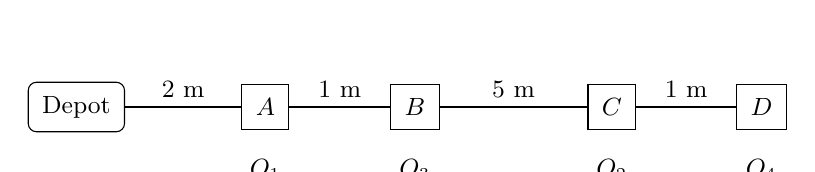
\begin{tikzpicture}[x=1cm,y=1cm,every node/.style={font=\small}]
\node[draw,rounded corners=3pt,inner sep=5pt] (depot) at (0,0) {Depot};
\node[draw,inner sep=5pt] (a) at (2.4,0) {$A$};
\node[draw,inner sep=5pt] (b) at (4.3,0) {$B$};
\node[draw,inner sep=5pt] (c) at (6.8,0) {$C$};
\node[draw,inner sep=5pt] (d) at (8.7,0) {$D$};
\draw (depot)--node[above]{2 m}(a);
\draw (a)--node[above]{1 m}(b);
\draw (b)--node[above]{5 m}(c);
\draw (c)--node[above]{1 m}(d);
\node[below=0.25cm of a] {$O_1$};
\node[below=0.25cm of b] {$O_3$};
\node[below=0.25cm of c] {$O_2$};
\node[below=0.25cm of d] {$O_4$};
\end{tikzpicture}
\caption{Đồ thị lối đi của ví dụ bốn đơn.}\label{fig:model-example}
\end{figure}

Mỗi đơn yêu cầu một đơn vị sản phẩm, có tải $1$ và thời gian lấy $1$ phút. Sức chứa xe $Q=2$, vận tốc $v=2$ mét/phút, thời gian chuẩn bị $b=1$ phút và thời gian thao tác tại vị trí $h_{\rm loc}=0$. Thứ tự đầu vào là $O_1,O_2,O_3,O_4$; hạn và vị trí của từng đơn được cho trong \tabref{tab:example-orders}.

\begin{table}[H]
\centering\small
\begin{tabular}{llrr}
\toprule
Đơn & Vị trí sản phẩm & Tải & Hạn, phút \\
\midrule
$O_1$ & $A$ & 1 & 7 \\
$O_2$ & $C$ & 1 & 12 \\
$O_3$ & $B$ & 1 & 7 \\
$O_4$ & $D$ & 1 & 12 \\
\bottomrule
\end{tabular}
\caption{Đơn hàng trong ví dụ minh họa.}\label{tab:example-orders}
\end{table}

B0 gom theo thứ tự thành hai chuyến $\{O_1,O_2\}$ và $\{O_3,O_4\}$, giao cho hai nhân viên và cùng bắt đầu tại $0$. Chuyến thứ nhất đi đến $C$ rồi quay về, với điểm dừng $d_0\to A\to C\to d_0$ và quãng đường $2+6+8=16$ mét. Theo \eqref{eq:model-duration}, thời lượng là $1+16/2+2=11$ phút. Chuyến thứ hai có quãng đường $3+6+9=18$ mét và thời lượng $1+18/2+2=12$ phút.

Vì đơn hoàn thành khi chuyến quay về, $O_1$ trễ $11-7=4$ phút và $O_3$ trễ $12-7=5$ phút; hai đơn còn lại đúng hạn. Nghiệm B0 vẫn khả thi vì mỗi chuyến có tải $2$ và đủ bốn đơn. Các chỉ tiêu là $D=34$, $C_{\max}=12$, $T=9$, $L=2$ và $R_{\rm on}=50\%$. Thang chuẩn hóa là $D_{\rm ref}=34$, $C_{\rm ref}=12$ và $T_{\rm ref}=4\times12=48$.

Với trọng số bằng nhau, điểm của B0 được tính bởi
\begin{equation}
 F(B0)=\frac13\left(\frac{34}{34}+\frac{12}{12}+\frac9{48}\right)
 =\frac{35}{48}\approx0{,}729167.\label{eq:model-example-b0}
\end{equation}

Trên cùng đầu vào, Greedy Batching (B2) tạo hai chuyến $\{O_1,O_3\}$ và $\{O_2,O_4\}$ trong cài đặt hiện tại. Chuyến gần depot có quãng đường $2+1+3=6$ mét và thời lượng $1+6/2+2=6$ phút. Chuyến xa có quãng đường $8+1+9=18$ mét và thời lượng $12$ phút. Mỗi nhân viên nhận một chuyến; cả bốn đơn đều đúng hạn.

Để minh họa riêng ảnh hưởng của lập lịch, xét phương án $X$ giữ nguyên hai chuyến và tuyến của B2 nhưng giao cả hai cho nhân viên thứ nhất, thực hiện chuyến gần trước. Nhân viên thứ hai không nhận chuyến. Chuyến đầu bắt đầu tại $0$ và kết thúc tại $6$; chuyến sau bắt đầu tại $6$ và kết thúc tại $18$ phút. Hai đơn gần depot vẫn đúng hạn, còn $O_2,O_4$ cùng trễ $18-12=6$ phút. Vì vậy $D=24$, $C_{\max}=18$, $T=12$ và $L=2$. Đây là phương án phân công khác dùng để minh họa, không phải đầu ra của B2.

\begin{table}[H]
\centering\small
\begin{tabular}{lrrrrr}
\toprule
Phương án & $D$, m & $C_{\max}$, phút & $T$, phút & $L$ & $F$ \\
\midrule
B0 & 34 & 12 & 9 & 2 & 0,729167 \\
B2 & 24 & 12 & 0 & 0 & 0,568627 \\
$X$, một nhân viên & 24 & 18 & 12 & 2 & 0,818627 \\
\bottomrule
\end{tabular}
\caption{So sánh các chỉ tiêu của ba phương án trong ví dụ.}\label{tab:example-comparison}
\end{table}

Dùng cùng thang chuẩn hóa của B0, điểm của B2 là
\begin{equation}
 F(B2)=\frac13\left(\frac{24}{34}+\frac{12}{12}+\frac0{48}\right)
 =\frac{29}{51}\approx0{,}568627.\label{eq:model-example-b2}
\end{equation}
Theo \tabref{tab:example-comparison}, B2 giảm $10$ mét, giữ nguyên makespan và loại độ trễ trong ví dụ. Mức giảm mục tiêu so với B0 là
\begin{equation}
 100\frac{F(B0)-F(B2)}{F(B0)}\approx22{,}02\%.\label{eq:model-example-improvement}
\end{equation}
Dùng cùng thang chuẩn hóa của B0, điểm của phương án $X$ là
\begin{equation}
 F(X)=\frac13\left(\frac{24}{34}+\frac{18}{12}+\frac{12}{48}\right)
 =\frac{167}{204}\approx0{,}818627.\label{eq:model-example-sequential}
\end{equation}
So với B2, phương án $X$ giữ nguyên quãng đường nhưng có makespan và độ trễ lớn hơn do dồn hai chuyến vào một nhân viên. Ví dụ này làm rõ rằng đánh giá cách gom đơn và tuyến đi cần đi cùng đánh giá phân công và lịch thực hiện.

Ví dụ cho thấy cách tính các nghiệm khả thi và các thành phần mục tiêu. Cả ba phương án đã được đánh giá và kiểm chứng chỉ tiêu bằng chương trình, nhưng không được cộng vào benchmark hoặc dùng làm bằng chứng về ưu thế trên toàn bộ dữ liệu. Ví dụ cũng không chứng minh B2 đạt tối ưu toàn cục; cơ chế tạo hai cách gom được giải thích tiếp ở Chương 3.

\clearpage
\section{THIẾT KẾ VÀ PHÂN TÍCH CÁC THUẬT TOÁN}
\label{sec:chuong3}

\subsection{Quy trình giải bài toán}
Chương này trình bày cách năm phương pháp được áp dụng vào mô hình ở Chương 2: First-Come, First-Served Batching (B0), Greedy Batching (B2), Large Neighborhood Search (LNS), Adaptive Large Neighborhood Search (ALNS) và Variable Neighborhood Search (VNS). Cấu trúc nghiệm là danh sách chuyến của từng nhân viên trong \eqref{eq:model-plan}; chất lượng được tính bằng \eqref{eq:model-objective}. Các phương pháp khác nhau ở cách tạo và thay đổi nghiệm, nhưng dùng cùng các đại lượng quãng đường, makespan và độ trễ.

Quy trình bắt đầu bằng kiểm tra đầu vào, tính khoảng cách trên đồ thị và xây dựng B0 để cố định thang chuẩn hóa. Nếu chọn B0, chương trình sử dụng nghiệm này làm đầu ra. Các phương pháp còn lại tạo B2; riêng LNS, ALNS và VNS tiếp tục cải thiện từ B2. Sau cùng, chương trình xuất tuyến, lịch, chỉ tiêu và kiểm chứng chúng trước khi trả kết quả.

\begin{figure}[H]
\centering
\begin{tikzpicture}[node distance=0.55cm,every node/.style={font=\small}]
\node[chthreeblue,text width=9cm] (input) {Kiểm tra đầu vào, tính khoảng cách và tạo B0 làm mốc};
\node[chthreegreen,text width=9cm,below=of input] (initial) {Chọn B0 hoặc khởi tạo B2};
\node[chthreepurple,text width=9cm,below=of initial] (search) {LNS, ALNS hoặc VNS cải thiện nghiệm từ B2};
\node[chthreeblue,text width=9cm,below=of search] (decode) {Xuất tuyến, lịch và các chỉ tiêu};
\node[chthreeorange,text width=9cm,below=of decode] (check) {Kiểm chứng kết quả và trả nghiệm};
\draw[chthreeflow] (input)--(initial);
\draw[chthreeflow] (initial)--node[right]{Tìm kiếm}(search);
\draw[chthreeflow] (search)--(decode);
\draw[chthreeflow] (decode)--(check);
\draw[chthreedash] (initial.west)--++(-0.8,0)|-node[pos=0.7,left]{B0/B2}(decode.west);
\end{tikzpicture}
\caption{Quy trình giải và kiểm chứng của năm phương pháp.}\label{fig:solver-flow}
\end{figure}

Ngân sách tìm kiếm của LNS, ALNS và VNS được tính từ trước khi tạo B2, nên bao gồm khởi tạo và tìm kiếm. Tiền xử lý, tạo mốc B0 và kiểm chứng đầu ra được đo riêng. Chương trình dừng theo ngân sách thời gian hoặc số vòng tối đa; các điểm kiểm tra thời gian không ngắt tức thời một phép dựng tuyến hoặc đánh giá đang thực hiện. Vì vậy, thời gian chạy tổng không được đồng nhất với ngân sách tìm kiếm, cũng không phải makespan của kế hoạch.

\subsection{Định tuyến, lập lịch và đánh giá nghiệm}

\subsubsection{Xây dựng tuyến bằng Nearest Neighbor}
Với tập vị trí $U(B)$ của một chuyến, Nearest Neighbor bắt đầu tại depot. Tại mỗi bước, thuật toán chọn vị trí chưa phục vụ gần nhất theo khoảng cách đường đi ngắn nhất $\delta$; mã vị trí dùng để phá hòa. Sau khi phục vụ các vị trí yêu cầu ngoài depot, tuyến quay về depot. Dãy điểm dừng được mở rộng thành đường đi trên đồ thị như đã mô tả ở mục 2.2.

Quy tắc chọn tại điểm $u$ có thể viết
\begin{equation}
 u^*=\arg\min_{z\in U_{\rm remaining}}(\delta(u,z),\operatorname{id}(z)).\label{eq:nn-choice}
\end{equation}
Đây là lựa chọn tham lam từng bước, không bảo đảm tuyến ngắn nhất trên toàn bộ tập vị trí. Với $r$ vị trí ngoài depot và tra cứu khoảng cách đã có, việc chọn thứ tự điểm dừng cần $O(r^2)$ phép xét. Chi phí mở rộng đường đi vật lý được tính thêm theo độ dài dãy đỉnh xuất ra. B0 dùng trực tiếp quy tắc này; bốn phương pháp còn lại kết hợp với 2-Opt.

\subsubsection{Cải thiện tuyến bằng 2-Opt}
2-Opt xét hai cạnh $(a,b)$ và $(c,d)$ trong tuyến. Trên đồ thị vô hướng, đảo đoạn giữa $b$ và $c$ thay hai cạnh này bằng $(a,c)$ và $(b,d)$. Độ thay đổi quãng đường là
\begin{equation}
 \Delta_D=\delta(a,c)+\delta(b,d)-\delta(a,b)-\delta(c,d).\label{eq:two-opt-delta}
\end{equation}
Trong cài đặt, một biến đổi được nhận nếu $\Delta_D<-10^{-9}$. Thuật toán nhận cặp cải thiện đầu tiên theo thứ tự vòng lặp, đảo đoạn rồi bắt đầu lượt quét mới. Quá trình kết thúc khi một lượt quét không tìm thấy cải thiện; depot được giữ ở hai đầu tuyến.

Nếu $\rho$ là số lần đảo đoạn được nhận, chi phí xét cặp là $O((\rho+1)r^2)$, bao gồm lượt cuối không cải thiện. Đảo một đoạn còn cần $O(r)$ thao tác. Không xem $\rho$ là hằng số hoặc mặc định số lượt cải thiện có cận đa thức theo $r$. Điều kiện dừng chỉ cho biết không còn cải thiện bằng phép đổi đang xét trong dung sai, không chứng minh tuyến tối ưu toàn cục.

\subsubsection{Phân công nhân viên và xây dựng lịch thực hiện}
Sau bước gom đơn cơ sở, các chuyến được sắp theo hạn nhỏ nhất của các đơn thành viên. Khi bằng nhau, chương trình giữ thứ tự chỉ số chuyến đã tạo. Lần lượt từng chuyến được giao cho nhân viên có thời điểm rảnh sớm nhất; mã nhân viên dùng để phá hòa. Thời điểm rảnh được cập nhật bằng thời lượng chuyến trong \eqref{eq:model-duration}.

Nếu có $b_{
m trip}$ chuyến, xác định hạn nhỏ nhất cần xét tổng cộng $n$ đơn; sắp chuyến cần $O(b_{
m trip}\log b_{
m trip})$, còn lựa chọn nhân viên bằng quét danh sách cần $O(b_{
m trip}m)$. Chi phí tính thời lượng và tuyến được cộng riêng. Quy tắc gom theo thứ tự của B0 vì vậy không đồng nghĩa với việc mọi chuyến được thực hiện theo thứ tự đơn đến.

Trong tìm kiếm, phân công và thứ tự chuyến là một phần của nghiệm, có thể được thay đổi trực tiếp. Chương trình không tự sắp lại tất cả chuyến theo hạn sau mỗi biến đổi, vì thao tác đó có thể xóa quyết định lập lịch vừa tạo. Lịch được tính lại theo từng danh sách chuyến bằng \eqref{eq:model-schedule}.

\subsubsection{Tính giá trị mục tiêu và kiểm tra ràng buộc}
Một ứng viên hoàn chỉnh phải phục vụ đủ đơn, không trùng đơn và đúng sức chứa trước khi được xem là nghiệm đầu ra. Bộ đánh giá dựng tuyến theo chế độ đang dùng, tính thời lượng, lịch và các thành phần trong $F$. Khi một chuyến thay đổi, thời điểm của các chuyến phía sau cùng nhân viên cũng có thể thay đổi; không chỉ tính chi phí riêng của đơn vừa di chuyển.

Trong phá hủy--tái thiết, bộ đánh giá có thể nhận trạng thái tạm thiếu đơn để xếp hạng hành động chèn. Khi đó, chỉ tiêu chỉ được tính trên các đơn đang có trong trạng thái, nhưng thang chuẩn hóa vẫn cố định từ B0 của đầu vào đầy đủ. Điểm của trạng thái tạm không được coi là chất lượng một nghiệm hoàn chỉnh hoặc cận dưới đã chứng minh của bài toán.

Tuyến, thông tin chuyến và các tiền tố lịch được lưu trong bộ nhớ đệm để tái sử dụng khi cấu trúc tương ứng không đổi. Sau khi chọn đầu ra, bộ kiểm chứng đối chiếu đường đi, tải, thời gian và chỉ tiêu từ kết quả xuất ra. Cách tổ chức này gắn giá trị mục tiêu với kế hoạch thực sự được trình bày, thay vì chỉ tin vào một điểm số trung gian.

\subsection[First-Come, First-Served Batching]{First-Come, First-Served Batching (B0)}

\subsubsection{Ý tưởng và nguyên lý}
B0 tạo nghiệm cơ sở bằng cách duyệt các đơn theo thứ tự đầu vào. Chương trình sắp theo trường thứ tự, rồi theo mã đơn nếu bằng nhau. Mỗi đơn được thêm vào chuyến hiện tại nếu vừa sức chứa; nếu không, chuyến hiện tại được đóng và một chuyến mới được mở. Đầu vào bảo đảm từng đơn riêng lẻ vừa xe, nên bước này có thể phục vụ đủ đơn mà không cần tách đơn.

B0 không lựa chọn đơn theo độ gần vị trí hoặc mức giảm mục tiêu. Tuyến mỗi chuyến dùng Nearest Neighbor, còn phân công chuyến dùng quy tắc ở mục 3.2.3. Vai trò của B0 là cung cấp một kế hoạch dễ giải thích và mốc chuẩn hóa nhất quán, không phải một cận tối ưu.

\subsubsection{Các bước thực hiện và giả mã}
\begin{table}[H]
\centering\small
\begin{tabularx}{\linewidth}{rX}
\toprule
Bước & Thao tác \\
\midrule
 & Đầu vào: tập đơn, tải đơn, sức chứa, đồ thị và thông số vận hành. Đầu ra: nghiệm B0. \\
1 & Sắp đơn theo thứ tự đầu vào; phá hòa bằng mã đơn. \\
2 & Khởi tạo danh sách chuyến rỗng, chuyến hiện tại $B=\varnothing$ và tải $w=0$. \\
3 & Với mỗi đơn $i$, nếu $B\neq\varnothing$ và $w+w_i>Q$ thì lưu $B$, đặt $B=\varnothing$ và $w=0$. \\
4 & Thêm $i$ vào $B$ và cập nhật tải. \\
5 & Sau khi duyệt hết đơn, lưu chuyến cuối nếu không rỗng. \\
6 & Tạo tuyến bằng Nearest Neighbor; sắp chuyến theo hạn nhỏ nhất và giao cho nhân viên rảnh sớm nhất. \\
7 & Tính lịch, chỉ tiêu, thang chuẩn hóa; kiểm chứng và trả nghiệm. \\
\bottomrule
\end{tabularx}
\caption{Giả mã B0 theo cài đặt của đề tài.}\label{tab:b0-pseudocode}
\end{table}
Các phép kiểm tra sức chứa trong mã có dùng dung sai số thực; giả mã viết điều kiện toán học để làm rõ ý tưởng. Các bước giải mã và kiểm chứng được tách ra để không lặp toàn bộ công thức của Chương 2.

\subsubsection{Ví dụ minh họa}
Với ví dụ ở mục 2.7, thứ tự đầu vào là $O_1,O_2,O_3,O_4$ và xe chứa được hai đơn. B0 tạo hai chuyến $\{O_1,O_2\}$ và $\{O_3,O_4\}$. Hai chuyến cùng có hạn nhỏ nhất là $7$ phút, nên được xét theo thứ tự tạo và giao cho hai nhân viên. Quãng đường lần lượt là $16$ và $18$ mét; thời lượng là $11$ và $12$ phút.

Theo \tabref{tab:example-comparison}, B0 có $D=34$, $C_{\max}=12$, $T=9$ và $F\approx0{,}729167$. Việc ghép đơn gần depot với đơn xa làm các đơn có hạn gần phải chờ chuyến quay về. Ví dụ minh họa hạn chế của quy tắc gom theo thứ tự trên đầu vào này, không khẳng định B0 kém hơn trên mọi bài.

\subsubsection{Phân tích chi phí tính toán và đặc điểm thuật toán}
Sắp đơn cần $O(n\log n)$, còn duyệt tải và tạo chuyến cần $O(n)$. Cần cộng chi phí lập lịch và dựng tuyến cho từng chuyến; do đó, không mô tả toàn bộ B0 chỉ bằng $O(n\log n)$. Chi phí tiền xử lý đồ thị được trình bày riêng ở mục 3.8.

B0 tất định với cùng đầu vào và quy tắc phá hòa. Nó dễ tái lập, tạo nghiệm khả thi theo sức chứa và ít quyết định tìm kiếm, nhưng không trực tiếp tối ưu quan hệ giữa vị trí, hạn và tải công việc. Giá trị của B0 nằm ở vai trò mốc so sánh và kiểm tra, không phải bảo đảm chất lượng gần tối ưu.

\subsection[Greedy Batching]{Greedy Batching (B2)}

\subsubsection{Ý tưởng và nguyên lý}
B2 chọn đơn có hạn sớm nhất trong tập chưa phục vụ làm hạt giống; mã đơn dùng để phá hòa. Trong các đơn còn vừa sức chứa, thuật toán chọn đơn làm tăng ít nhất quãng đường Nearest Neighbor của chuyến. Quy tắc được lặp đến khi không còn đơn vừa tải, rồi mở chuyến mới.

Gọi $B$ là chuyến đang tạo, tiêu chí thêm đơn là
\begin{equation}
 \Delta_i^{\rm NN}=D_{\rm NN}(B\cup\{i\})-D_{\rm NN}(B),\qquad
 i^*=\arg\min_{i:\,\text{vừa tải}}(\Delta_i^{\rm NN},d_i,\operatorname{id}(i)).\label{eq:greedy-batching-choice}
\end{equation}
Hạn chỉ quyết định hạt giống và phá hòa của bước chọn này. B2 chưa xét trực tiếp toàn bộ $F$ khi ghép đơn. Sau khi gom, chương trình dùng Nearest Neighbor kết hợp 2-Opt để tạo tuyến cuối, rồi phân công và lập lịch như mục 3.2.3. Cần phân biệt tiêu chí gom dựa trên tuyến Nearest Neighbor với tuyến đã được cải thiện của nghiệm xuất ra.

\subsubsection{Các bước thực hiện và giả mã}
\begin{table}[H]
\centering\small
\begin{tabularx}{\linewidth}{rX}
\toprule
Bước & Thao tác \\
\midrule
 & Đầu vào: các dữ liệu của B0 và thang chuẩn hóa cố định. Đầu ra: nghiệm B2. \\
1 & Khởi tạo tập đơn chưa phục vụ $R=O$ và danh sách chuyến rỗng. \\
2 & Khi $R\neq\varnothing$, lấy đơn có $(d_i,\operatorname{id}(i))$ nhỏ nhất làm chuyến $B$ và bỏ khỏi $R$. \\
3 & Lập tập các đơn trong $R$ có thể thêm vào $B$ mà không vượt tải. \\
4 & Nếu tập này rỗng, lưu $B$ và quay lại bước 2. \\
5 & Tính $\Delta_i^{\rm NN}$ cho từng đơn khả thi; chọn theo \eqref{eq:greedy-batching-choice}. \\
6 & Thêm đơn đã chọn vào $B$, bỏ khỏi $R$ và quay lại bước 3. \\
7 & Dựng tuyến cuối bằng Nearest Neighbor và 2-Opt; phân công, lập lịch, đánh giá và kiểm chứng. \\
\bottomrule
\end{tabularx}
\caption{Giả mã B2 theo cài đặt của đề tài.}\label{tab:b2-pseudocode}
\end{table}

\subsubsection{Ví dụ minh họa}
Trong ví dụ bốn đơn, $O_1$ và $O_3$ cùng có hạn $7$ phút; B2 chọn $O_1$ do mã nhỏ hơn. Chuyến đơn $\{O_1\}$ có quãng đường $4$ mét. Thêm $O_3$ làm quãng đường thành $6$ mét, tăng $2$ mét; thêm $O_2$ làm thành $16$ mét, tăng $12$ mét; thêm $O_4$ làm thành $18$ mét, tăng $14$ mét. Cả ba đều vừa tải, nên B2 ghép $O_3$ vào chuyến đầu.

Xe đã đầy, nên $O_2$ và $O_4$ được gom ở chuyến sau. Phân công mỗi nhân viên một chuyến tạo phương án B2 trong \tabref{tab:example-comparison}, với $D=24$, $C_{\max}=12$, $T=0$ và $F\approx0{,}568627$. Trên lối đi này, 2-Opt không làm giảm thêm quãng đường. Vì vậy, phần giảm đường đi trong riêng ví dụ đến từ cách gom; điều này không được suy rộng cho mọi so sánh B0--B2.

\subsubsection{Phân tích chi phí tính toán và đặc điểm thuật toán}
Mỗi lần thêm đơn có thể xét nhiều đơn còn lại. Với tối đa $n$ lần lựa chọn và tối đa $n$ ứng viên mỗi lần, số lượt tính phương án thêm có cận $O(n^2)$. Mỗi lượt vẫn cần xác định vị trí và quãng đường chuyến; sắp các đơn còn lại theo mã còn tạo chi phí riêng. Khi gọi $\mathcal C_{\rm cand}$ là chi phí tính một ứng viên gom, phần kiến tạo có cận dạng $O(n^2(\log n+\mathcal C_{\rm cand}))$, chưa gồm tuyến cuối và lập lịch.

B2 tất định và xét độ gần của nhóm đơn, nhưng tiêu chí tham lam cục bộ không trực tiếp tối thiểu hóa $F$. Một phép ghép tiết kiệm đường đi có thể làm tăng thời điểm hoàn thành hoặc trễ hạn. B2 do đó không được bảo đảm luôn tốt hơn B0. Vai trò tiếp theo của B2 là nghiệm khởi tạo khả thi để LNS, ALNS và VNS có một mốc xuất phát chung.

\subsection[Large Neighborhood Search]{Large Neighborhood Search (LNS)}

\subsubsection{Ý tưởng và nguyên lý}
LNS cải thiện một nghiệm bằng cách loại bỏ một phần các đơn rồi chèn chúng trở lại để tạo cấu trúc khác. Nguyên lý này kế thừa hướng tìm kiếm lân cận lớn của Shaw \cite{shaw1998}; các thao tác và tiêu chí chèn dưới đây mô tả riêng cài đặt của đề tài. LNS bắt đầu từ B2, lưu nghiệm hiện tại $X$ và nghiệm tốt nhất $X^*$ riêng biệt. Các toán tử phá hủy và tái thiết được chọn với trọng số bằng nhau.

Cấu hình dùng trong thực nghiệm chính có bốn toán tử phá hủy. Random Removal lấy mẫu đơn ngẫu nhiên. Related Removal chọn một đơn hạt giống $i_0$ rồi xếp các đơn theo mức liên quan
\begin{equation}
 r(i_0,i)=\frac{\min_{u\in U(\{i_0\}),z\in U(\{i\})}\delta(u,z)}{D_{\rm ref}}
 +\frac{|d_{i_0}-d_i|}{C_{\rm ref}},\label{eq:related-removal}
\end{equation}
phá hòa bằng mã đơn. Late Removal ưu tiên độ trễ giảm dần, rồi hạn và mã đơn. Batch Removal chọn một chuyến ngẫu nhiên và lấy toàn bộ đơn của chuyến đó ra. Các chuyến rỗng sau phá hủy được loại khỏi danh sách.

Với ba toán tử đầu, số đơn rút là
\begin{equation}
 q=\min\{n,q_{\max},\max(1,\lceil\eta n\rceil)\}.\label{eq:removal-size}
\end{equation}
Trong cấu hình chính, $\eta=0{,}15$ và $q_{\max}=6$. Batch Removal là ngoại lệ: nó bỏ cả chuyến, nên số đơn rút thực tế có thể lớn hơn $q_{\max}$. Cần dùng số đơn thực sự bị rút khi phân tích chi phí tái thiết.

Một hành động tái thiết có thể chèn đơn vào chuyến còn vừa tải, hoặc tạo chuyến mới tại một vị trí trong lịch của một nhân viên. Mỗi hành động được đánh giá bằng mục tiêu trên trạng thái tạm. Nếu số hành động vượt giới hạn ứng viên, cài đặt chọn ngẫu nhiên một hành động tạo chuyến mới bắt buộc và lấy mẫu các hành động còn lại. Cách này duy trì khả năng chèn lại một đơn riêng lẻ vừa xe, nhưng không bảo đảm xét hành động tốt nhất trong toàn bộ không gian. Phần chính dùng lấy mẫu uniform; giới hạn $24$ áp dụng cho từng đơn đang xét, không phải cho toàn bộ lần tái thiết.

Hai quy tắc tái thiết dùng chung các hành động trên. Greedy Repair chọn đơn có điểm chèn tốt nhất nhỏ nhất. Regret-2 Repair ưu tiên đơn có chênh lệch lớn nhất giữa hai lựa chọn tốt nhất:
\begin{equation}
 R_i=c_{i,2}-c_{i,1},\qquad c_{i,1}\leq c_{i,2}.\label{eq:regret-two}
\end{equation}
Sau khi chọn đơn, cả hai quy tắc thực hiện hành động tốt nhất của đơn đó, cập nhật trạng thái và đánh giá lại các đơn còn chờ. Nếu chỉ có một hành động, cài đặt đặt regret bằng vô cùng để ưu tiên đơn này. Các giá trị regret dựa trên danh sách ứng viên đã giữ, không nhất thiết dựa trên tất cả vị trí chèn có thể có.

Mỗi năm vòng hoàn chỉnh trong cấu hình chính, ứng viên còn được cải thiện cục bộ với tối đa tám lần thử. Mỗi lần lấy mẫu chuyển/đổi đơn giữa hai chuyến hoặc đổi/chuyển một chuyến trong lịch. Chỉ biến đổi cải thiện $F$ mới được nhận trong bước cục bộ. Đây là bước có giới hạn số mẫu, không phải duyệt hết lân cận.

Ứng viên hoàn chỉnh được xét chấp nhận theo cơ chế Simulated Annealing \cite{kirkpatrick1983}. Đặt $\Delta=F(Y)-F(X)$ và gọi $\theta$ là nhiệt độ tìm kiếm, khác với tổng độ trễ $T$ ở Chương 2:
\begin{equation}
 P_{\rm accept}(Y\mid X)=
 \begin{cases}1,&\Delta\leq0,\\
 \exp\!\left(-\Delta/\max(\theta,10^{-12})\right),&\Delta>0.
 \end{cases}\label{eq:sa-acceptance}
\end{equation}
Nhiệt độ giảm sau mỗi vòng hoàn chỉnh theo $\theta\leftarrow\gamma\theta$, với $0<\gamma<1$. Việc cho phép nhận ứng viên xấu giúp thay đổi đường tìm kiếm, nhưng không bảo đảm thoát mọi cực trị hoặc tìm được tối ưu trong ngân sách hữu hạn.

\subsubsection{Các bước thực hiện và giả mã}
\begin{table}[H]
\centering\small
\begin{tabularx}{\linewidth}{rX}
\toprule
Bước & Thao tác \\
\midrule
 & Đầu vào: B2, thang chuẩn hóa, seed, toán tử và điều kiện dừng. Đầu ra: nghiệm tốt nhất đã lưu. \\
1 & Đặt $X=X^*=B2$; tính điểm và khởi tạo nhiệt độ. \\
2 & Khi còn số vòng và ngân sách, chọn một toán tử phá hủy và một toán tử tái thiết với trọng số bằng nhau. \\
3 & Rút các đơn đã chọn khỏi $X$, loại chuyến rỗng để tạo trạng thái tạm. \\
4 & Đánh giá các hành động chèn; dùng Greedy Repair hoặc Regret-2 Repair đến khi chèn lại đủ đơn. \\
5 & Nếu đến chu kỳ cải thiện cục bộ, thực hiện các lần thử đã giới hạn; chỉ nhận cải thiện. \\
6 & Tính $F(Y)$ của ứng viên hoàn chỉnh. Nếu hết thời gian trong bước 3--5, bỏ lần đang thực hiện và chuyển đến bước 10. \\
7 & Chấp nhận $Y$ theo \eqref{eq:sa-acceptance}; nếu được nhận, đặt $X=Y$. \\
8 & Nếu $F(Y)<F(X^*)-10^{-12}$ thì lưu $X^*=Y$. \\
9 & Giảm nhiệt độ; chuyển sang vòng tiếp theo. Trọng số toán tử vẫn bằng $1$. \\
10 & Kiểm chứng và trả $X^*$, không trả trạng thái tạm thiếu đơn. \\
\bottomrule
\end{tabularx}
\caption{Giả mã LNS với lựa chọn toán tử đều.}\label{tab:lns-pseudocode}
\end{table}
Giả mã tách bước chấp nhận nghiệm hiện tại và bước ghi nhận nghiệm tốt nhất như cài đặt. Việc nhận một ứng viên xấu không xóa nghiệm tốt nhất đã có. Số vòng hoàn chỉnh có thể bằng $0$ nếu ngân sách đã hết sau khởi tạo.

\subsubsection{Ví dụ minh họa}
Để minh họa bước tái thiết trên dữ liệu ở mục 2.7, lấy $O_2,O_3$ ra khỏi phương án B0. Trạng thái còn lại có $\{O_1\}$ ở nhân viên thứ nhất và $\{O_4\}$ ở nhân viên thứ hai. Đây là một trạng thái minh họa cho thao tác, không phải tuyên bố rằng LNS khởi tạo từ B0; trong lượt giải chính, LNS khởi tạo từ B2.

Với các hành động được xét đầy đủ trên bài nhỏ, hai điểm tốt nhất của mỗi đơn cần chèn là:
\begin{table}[H]
\centering\small
\begin{tabular}{lrrr}
\toprule
Đơn & Điểm tốt nhất $c_{i,1}$ & Điểm thứ hai $c_{i,2}$ & Regret \\
\midrule
$O_2$ & 0,549020 & 0,666667 & 0,117647 \\
$O_3$ & 0,540850 & 0,583742 & 0,042892 \\
\bottomrule
\end{tabular}
\caption{Các lựa chọn chèn trong ví dụ tái thiết hai đơn.}\label{tab:repair-example}
\end{table}
Greedy Repair chèn $O_3$ trước vì điểm tốt nhất nhỏ hơn; Regret-2 Repair chèn $O_2$ trước vì regret lớn hơn. Sau khi cập nhật và chèn đơn còn lại, cả hai cùng tạo các chuyến $\{O_1,O_3\}$ và $\{O_2,O_4\}$ với $F\approx0{,}568627$. Ví dụ làm rõ khác biệt trong thứ tự quyết định, không chứng minh hai quy tắc luôn cho cùng nghiệm hoặc quy tắc nào tốt hơn.

Nếu một ứng viên có $\Delta=0{,}02$ tại $\theta=0{,}03$, xác suất nhận theo \eqref{eq:sa-acceptance} là $\exp(-0{,}02/0{,}03)\approx0{,}5134$. Đây là phép tính minh họa cơ chế chấp nhận, không phải xác suất thành công của LNS trên benchmark.

\subsubsection{Phân tích chi phí tính toán và đặc điểm thuật toán}
Nếu một lần tái thiết rút $q$ đơn và xét tối đa $A$ hành động cho mỗi đơn đang chờ, số lượt đánh giá hành động có cận
\begin{equation}
 A\sum_{j=1}^{q}j=\frac{Aq(q+1)}2.\label{eq:repair-evaluation-bound}
\end{equation}
Trong cấu hình chính, có thể lấy $A=24$; khi tắt giới hạn ứng viên, phải dùng số vị trí chèn thực tế. Mỗi lượt còn tốn chi phí sao chép nghiệm, giải mã tuyến, tính lịch và kiểm tra ràng buộc. Lập danh sách, tính regret và sắp lựa chọn cũng có chi phí, nên số vòng tìm kiếm không đủ để phản ánh toàn bộ thời gian tính toán.

LNS có thể thay đổi nhiều đơn cùng lúc và xét ảnh hưởng lên cả ba thành phần mục tiêu. Tuy nhiên, chi phí tái thiết tăng theo số đơn rút; lấy mẫu ứng viên có thể bỏ lỡ vị trí tốt và Simulated Annealing cần tham số nhiệt độ. Trong dung sai ghi nhận nghiệm tốt nhất, đầu ra không kém B2 theo cùng bộ đánh giá. Tính chất này không bảo đảm tốt hơn một phương pháp tìm kiếm khác hoặc đạt tối ưu toàn cục.

\subsection[Adaptive Large Neighborhood Search]{Adaptive Large Neighborhood Search (ALNS)}

\subsubsection{Ý tưởng và nguyên lý}
ALNS dùng cùng toán tử phá hủy, tái thiết, cải thiện cục bộ và cơ chế chấp nhận như LNS, nhưng điều chỉnh xác suất chọn toán tử dựa trên kết quả đã quan sát. Hướng lựa chọn thích ứng tham khảo Ropke và Pisinger \cite{ropke2006}; thang thưởng và cập nhật dưới đây là các quy tắc của cài đặt đang được đánh giá.

Gọi $\omega_h>0$ là trọng số của toán tử $h$. Các toán tử phá hủy và tái thiết được chọn riêng trong từng nhóm $\mathcal D$ và $\mathcal R$:
\begin{equation}
 p_h=\frac{\omega_h}{\sum_{g\in\mathcal G}\omega_g},\qquad
 \mathcal G\in\{\mathcal D,\mathcal R\}.\label{eq:operator-probability}
\end{equation}
Ban đầu mọi trọng số bằng $1$. Sau một vòng hoàn chỉnh, cả toán tử phá hủy và tái thiết đã dùng nhận cùng một điểm thưởng theo kết quả của ứng viên:
\begin{table}[H]
\centering\small
\begin{tabularx}{\linewidth}{Xr}
\toprule
Kết quả của vòng tìm kiếm & Điểm thưởng \\
\midrule
Cải thiện nghiệm tốt nhất đã lưu & 8 \\
Được chấp nhận và cải thiện nghiệm hiện tại, nhưng chưa cải thiện tốt nhất & 3 \\
Được chấp nhận trong trường hợp còn lại & 1 \\
Không được chấp nhận & 0 \\
\bottomrule
\end{tabularx}
\caption{Điểm thưởng cho toán tử trong cài đặt ALNS.}\label{tab:operator-rewards}
\end{table}
Các điều kiện cải thiện dùng dung sai $10^{-12}$. Thưởng dựa trên ứng viên sau cả tái thiết và bước cục bộ nếu có; vì vậy nó là tín hiệu hiệu quả của một vòng kết hợp, không phải phép đo tác động độc lập của từng toán tử.

Sau một phân đoạn, gọi $N_h$ là số lần toán tử được dùng và $R_h$ là tổng thưởng trong đoạn. Với $N_h>0$, trọng số được cập nhật bởi
\begin{equation}
 \omega_h\leftarrow\max\left\{0{,}05,(1-\lambda)\omega_h+\lambda\frac{R_h}{N_h}\right\}.\label{eq:operator-weight-update}
\end{equation}
Toán tử chưa được dùng giữ nguyên trọng số; sau cập nhật, số lần dùng và tổng thưởng của đoạn được đặt lại bằng $0$. Sàn $0{,}05$ giữ xác suất dương, nhưng không bảo đảm mọi toán tử được chọn trong một lượt chạy hữu hạn. Chương trình cũng cập nhật phần thống kê còn lại khi kết thúc lượt giải.

\subsubsection{Các bước thực hiện và giả mã}
\begin{table}[H]
\centering\small
\begin{tabularx}{\linewidth}{rX}
\toprule
Bước & Thao tác \\
\midrule
 & Đầu vào: dữ liệu của LNS, độ dài phân đoạn và hệ số phản ứng. Đầu ra: nghiệm tốt nhất đã lưu. \\
1 & Đặt $X=X^*=B2$; khởi tạo nhiệt độ và mọi trọng số toán tử bằng $1$. \\
2 & Đặt thống kê số lần dùng và tổng thưởng của từng toán tử bằng $0$. \\
3 & Khi còn ngân sách và số vòng, chọn phá hủy và tái thiết theo \eqref{eq:operator-probability}. \\
4 & Phá hủy, tái thiết và cải thiện cục bộ định kỳ như LNS. \\
5 & Nếu hết thời gian trước khi hoàn tất ứng viên, bỏ vòng đang thực hiện và đến bước 12. \\
6 & Tính $F(Y)$, đặt $\Delta=F(Y)-F(X)$; xét chấp nhận theo \eqref{eq:sa-acceptance}. \\
7 & Nếu được nhận, cập nhật $X$ và thưởng $3$ khi cải thiện hiện tại, hoặc $1$ trong trường hợp còn lại. Nếu bị từ chối, thưởng $0$. \\
8 & Nếu cải thiện $X^*$, lưu nghiệm tốt nhất và thay thưởng bằng $8$. \\
9 & Cộng thưởng và tăng số lần dùng cho cả hai toán tử đã chọn. \\
10 & Khi hết phân đoạn, cập nhật trọng số theo \eqref{eq:operator-weight-update} và đặt lại thống kê đoạn. \\
11 & Giảm nhiệt độ; tiếp tục vòng sau. \\
12 & Cập nhật thống kê đoạn còn lại; kiểm chứng và trả $X^*$. \\
\bottomrule
\end{tabularx}
\caption{Giả mã ALNS với lựa chọn toán tử thích ứng.}\label{tab:alns-pseudocode}
\end{table}
Trong cấu hình của đợt benchmark chính, phân đoạn có $10$ vòng và $\lambda=0{,}25$. Cần phân biệt cấu hình thực nghiệm này với giá trị mặc định của lớp cấu hình. Nếu lượt chạy kết thúc trước một lần cập nhật được dùng cho các vòng tiếp theo, tác động của lựa chọn thích ứng có thể chưa xuất hiện trong quá trình tìm kiếm.

\subsubsection{Ví dụ minh họa}
Giả sử một toán tử có trọng số $1$, được dùng bốn lần trong đoạn và nhận tổng thưởng $12$. Với $\lambda=0{,}25$, cập nhật cho trọng số mới
\begin{equation}
 \omega_h'=\max\{0{,}05,0{,}75\times1+0{,}25\times12/4\}=1{,}5.\label{eq:operator-weight-example}
\end{equation}
Nếu ba toán tử phá hủy còn lại vẫn có trọng số $1$, xác suất chọn toán tử này trong nhóm tăng từ $1/4$ lên $1{,}5/4{,}5=1/3$. Ví dụ mô tả tác động của điểm thưởng lên xác suất, không kết luận toán tử đó luôn tạo nghiệm tốt.

Bước tái thiết của ALNS vẫn có thể dùng các lựa chọn trong \tabref{tab:repair-example}. Điểm khác LNS nằm ở cách chọn toán tử qua các đoạn, không nằm ở việc thay đổi hàm mục tiêu hoặc tự động chọn hành động chèn tốt nhất trong toàn bộ không gian. Khi các toán tử tạo cùng kết quả trên một bài nhỏ, hai phương pháp có thể trả cùng điểm mà chưa cho phép kết luận thích ứng vô ích trên mọi dữ liệu.

\subsubsection{Phân tích chi phí tính toán và đặc điểm thuật toán}
Chi phí tạo ứng viên của ALNS có cùng cấu trúc với LNS. Phần bổ sung là lấy mẫu theo trọng số, ghi thưởng và cập nhật các toán tử theo phân đoạn. Với số toán tử nhỏ và cố định, phần này thường nhỏ hơn chi phí dựng tuyến và đánh giá nhiều hành động chèn, nhưng mức chênh lệch thời gian cần được đo thay vì mặc định bằng không.

ALNS khai thác thông tin của các vòng đã chạy để thay đổi tần suất sử dụng toán tử. Hiệu quả phụ thuộc vào số vòng có thể hoàn thành, độ dài phân đoạn, hệ số phản ứng và đặc điểm đầu vào. LNS là đối chứng cho phần lựa chọn thích ứng khi giữ chung các thành phần khác. Trong ngân sách thời gian bằng nhau, số vòng và chuỗi ngẫu nhiên của hai phương pháp vẫn có thể khác; việc đánh giá cơ chế cần giữ phạm vi kết luận theo thiết kế thực nghiệm.

Như LNS, ALNS trả nghiệm tốt nhất đã ghi nhận, nên dãy điểm tốt nhất không tăng và đầu ra không kém nghiệm khởi tạo trong dung sai. Nghiệm hiện tại có thể xấu đi do cơ chế chấp nhận. Hai tính chất này cần được phân biệt khi đọc đường hội tụ; chúng không tạo bảo đảm tối ưu toàn cục hoặc ưu thế của ALNS so với VNS.

\subsection[Variable Neighborhood Search]{Variable Neighborhood Search (VNS)}

\subsubsection{Ý tưởng và nguyên lý}
VNS thay đổi cấu trúc lân cận để tìm kiếm từ nhiều cách biến đổi nghiệm, theo nguyên lý của Mladenović và Hansen \cite{mladenovic1997}. Cài đặt của đề tài bắt đầu từ B2, thực hiện rung lắc rồi cải thiện bằng một số mẫu lân cận có giới hạn. Nghiệm sau bước này chỉ thay thế nghiệm tốt nhất khi có cải thiện; VNS không dùng cơ chế Simulated Annealing của LNS và ALNS.

Ba nhóm lân cận được dùng là Order Neighborhood, Schedule Neighborhood và Batch Neighborhood. Nhóm thứ nhất chuyển một đơn giữa hai chuyến hoặc đổi hai đơn thuộc hai chuyến, với tải sau thay đổi không vượt sức chứa. Nhóm thứ hai đổi hai chuyến hoặc lấy một chuyến ra rồi chèn vào vị trí khác, có thể chuyển sang nhân viên khác. Nhóm thứ ba tách một phần đơn thành chuyến mới, hoặc gộp hai chuyến nếu tổng tải cho phép. Chuyến rỗng sau biến đổi được loại bỏ; thao tác không khả thi có thể trả lại nghiệm ban đầu.

Gọi $\kappa\in\{1,\ldots,6\}$ là mức rung lắc. Nhóm được chọn theo
\begin{equation}
 g=1+((\kappa-1)\bmod3),\label{eq:vns-shaking-group}
\end{equation}
và một lần rung lắc gọi nhóm đó $\kappa$ lần liên tiếp. Mức lớn hơn vì vậy tăng số thao tác được thử, không bảo đảm mỗi thao tác tạo ra một thay đổi khác biệt.

\begin{table}[H]
\centering\small
\begin{tabularx}{\linewidth}{lXl}
\toprule
Mức rung lắc & Nhóm lân cận & Số lần gọi \\
\midrule
$1,4$ & Chuyển hoặc đổi đơn giữa các chuyến & $1,4$ \\
$2,5$ & Đổi hoặc chuyển vị trí chuyến trong lịch & $2,5$ \\
$3,6$ & Tách hoặc gộp chuyến & $3,6$ \\
\bottomrule
\end{tabularx}
\caption{Quan hệ giữa mức rung lắc và nhóm lân cận của VNS.}\label{tab:vns-neighborhoods}
\end{table}

Sau rung lắc, bước cải thiện bắt đầu từ nhóm chuyển/đổi đơn. Nếu một mẫu làm giảm $F$ quá dung sai $10^{-12}$, ứng viên được cập nhật và việc chọn nhóm quay về nhóm đầu. Nếu không, chuyển tuần hoàn sang nhóm tiếp theo. Tổng số lần thử bị giới hạn bởi tham số cải thiện cục bộ; cấu hình chính dùng tám lần. Cách này là cải thiện trên mẫu, không phải duyệt hết lân cận hoặc xác nhận một cực trị cục bộ đầy đủ.

Nếu ứng viên cuối tốt hơn nghiệm tốt nhất, chương trình nhận ứng viên và đặt $\kappa=1$. Nếu không, giữ nghiệm tốt nhất và đặt $\kappa\leftarrow1+(\kappa\bmod6)$. Rung lắc có thể tạo ứng viên tạm xấu hơn, nhưng ứng viên đó không được trả như nghiệm tốt nhất chỉ vì đã được tạo ra.

\subsubsection{Các bước thực hiện và giả mã}
\begin{table}[H]
\centering\small
\begin{tabularx}{\linewidth}{rX}
\toprule
Bước & Thao tác \\
\midrule
 & Đầu vào: B2, seed, ba nhóm lân cận và điều kiện dừng. Đầu ra: nghiệm tốt nhất đã lưu. \\
1 & Đặt $X^*=B2$, tính $F(X^*)$ và khởi tạo $\kappa=1$. \\
2 & Khi còn ngân sách và số vòng, đặt ứng viên $Y=X^*$. \\
3 & Chọn nhóm $g$ theo \eqref{eq:vns-shaking-group}; áp dụng nhóm này $\kappa$ lần để rung lắc $Y$. \\
4 & Tính $F(Y)$ và đặt nhóm cải thiện $j=1$. \\
5 & Trong số lần thử cho phép, lấy một mẫu $Z$ từ nhóm $j$ của $Y$ và tính $F(Z)$. \\
6 & Nếu $F(Z)<F(Y)-10^{-12}$, đặt $Y=Z$ và $j=1$; nếu không, đặt $j=1+(j\bmod3)$. \\
7 & Nếu $F(Y)<F(X^*)-10^{-12}$, lưu $X^*=Y$ và đặt $\kappa=1$; nếu không, tăng mức tuần hoàn. \\
8 & Nếu phát hiện hết thời gian trong lần đang thực hiện, dừng và giữ nghiệm tốt nhất đã ghi nhận. \\
9 & Kiểm chứng và trả $X^*$. \\
\bottomrule
\end{tabularx}
\caption{Giả mã VNS với cải thiện lân cận trên số mẫu giới hạn.}\label{tab:vns-pseudocode}
\end{table}

\subsubsection{Ví dụ minh họa}
Phương án $X$ ở mục 2.7 giao hai chuyến $\{O_1,O_3\}$ và $\{O_2,O_4\}$ cho cùng một nhân viên. Một thao tác thuộc Schedule Neighborhood chuyển chuyến thứ hai sang nhân viên đang không có chuyến, giữ nguyên tập đơn và tuyến của hai chuyến. Khi đó, hai chuyến cùng bắt đầu tại $0$, makespan giảm từ $18$ xuống $12$ phút và tổng độ trễ giảm từ $12$ xuống $0$; quãng đường vẫn là $24$ mét.

Điểm mục tiêu giảm từ $0{,}818627$ xuống $0{,}568627$, chênh lệch $0{,}25$ với cùng thang chuẩn hóa. Đây là minh họa một thao tác lập lịch được hỗ trợ trong cài đặt, không phải mô tả một lượt VNS khởi tạo từ $X$. Lượt giải của VNS vẫn khởi tạo từ B2; ví dụ cho thấy vì sao lân cận phân công chuyến có thể hữu ích khi kế hoạch hiện tại mất cân bằng.

Trong ví dụ khác của cùng tập đơn, một bước chuyển/đổi đơn có thể thay đổi nhóm vị trí cần ghé; tách/gộp chuyến có thể thay đổi cả thời gian chuẩn bị và lịch. Các biến đổi này cần được so sánh bằng toàn bộ $F$, không chỉ bằng khoảng cách của một đơn hay một chuyến.

\subsubsection{Phân tích chi phí tính toán và đặc điểm thuật toán}
Một vòng VNS gọi tối đa sáu thao tác rung lắc và $\ell$ thao tác cải thiện, trong đó $\ell=8$ ở cấu hình chính. Sau rung lắc có một lượt tính điểm; mỗi mẫu cải thiện có thêm một lượt. Gọi $\mathcal C_N$ là chi phí tạo một biến đổi và $\mathcal C_F$ là chi phí đánh giá một nghiệm, phần tìm kiếm qua $I$ vòng có cận dạng
\begin{equation}
 O\!\left(I\left[(6+\ell)\mathcal C_N+(1+\ell)\mathcal C_F\right]\right).\label{eq:vns-cost}
\end{equation}
Chi phí khởi tạo, xuất và kiểm chứng được cộng riêng. $\mathcal C_N$ gồm sao chép cấu trúc, kiểm tra tải và chuẩn hóa danh sách đơn; $\mathcal C_F$ vẫn phụ thuộc vào tuyến, lịch và bộ nhớ đệm. Khi dừng theo thời gian, $I$ là số vòng thực sự hoàn thành, không phải luôn bằng giới hạn cấu hình. Nếu một vòng bị ngắt, chi phí đã thực hiện của vòng đó còn phải cộng vào thời gian chạy thực tế.

VNS tác động trực tiếp lên gom đơn và lịch, không cần tái chèn toàn bộ một tập đơn đã rút. Tuy nhiên, số mẫu hữu hạn có thể bỏ lỡ biến đổi tốt; một thao tác thất bại hoặc trả lại nghiệm cũ vẫn tiêu tốn thời gian. Nghiệm tốt nhất không bị thay bằng ứng viên xấu, nhưng việc tuần hoàn lân cận không tạo bảo đảm thoát mọi cực trị hoặc tìm tối ưu toàn cục.

\subsection{So sánh cơ chế và phân tích chi phí tính toán}
Các phương pháp được đối chiếu theo thành phần cài đặt, không chỉ theo tên gọi. \tabref{tab:method-mechanisms} cho thấy B2 và ba phương pháp tìm kiếm dùng chung bước định tuyến cuối; LNS và ALNS giữ chung cơ chế tạo ứng viên, còn VNS thay đổi cấu trúc tìm kiếm.

\begin{table}[H]
\centering\small
\begin{tabularx}{\linewidth}{lXXX}
\toprule
Phương pháp & Tạo nghiệm hoặc ứng viên & Định tuyến & Chấp nhận trong tìm kiếm \\
\midrule
B0 & Gom theo thứ tự đầu vào & Nearest Neighbor & Không có pha tìm kiếm \\
B2 & Gom tham lam theo hạn và tăng quãng đường & Nearest Neighbor và 2-Opt & Không có pha tìm kiếm \\
LNS & Phá hủy--tái thiết, chọn toán tử đều & Nearest Neighbor và 2-Opt & Simulated Annealing; lưu tốt nhất riêng \\
ALNS & Phá hủy--tái thiết, chọn toán tử thích ứng & Nearest Neighbor và 2-Opt & Như LNS; thêm cập nhật trọng số \\
VNS & Rung lắc và cải thiện trên mẫu lân cận & Nearest Neighbor và 2-Opt & Chỉ cập nhật tốt nhất khi cải thiện \\
\bottomrule
\end{tabularx}
\caption{Đối chiếu các thành phần của năm phương pháp.}\label{tab:method-mechanisms}
\end{table}

Gọi $N_V=|V|$, $N_E=|E|$ và $h$ là số vị trí nguồn được tiền xử lý, gồm depot và các vị trí sản phẩm phân biệt. Với cách dùng Dijkstra trong chương trình, chi phí tiền xử lý khoảng cách có dạng $O(h(N_V+N_E)\log N_V)$, còn bảng khoảng cách và truy vết dùng bộ nhớ $O(hN_V)$ ngoài đồ thị. Phần này phục vụ chung các lần tính tuyến trong một lượt giải, không được coi là chi phí bằng không.

Để mô tả chi phí còn lại, gọi $\mathcal C_B(B)$ là chi phí tính thông tin một chuyến, gồm vị trí cần ghé, tải, tuyến và thời lượng; $\mathcal C_E$ là chi phí tạo và chấm một hành động chèn; $\mathcal C_F$ là chi phí chấm nghiệm. Các đại lượng này phụ thuộc kích thước chuyến, số điểm lấy hàng, số lần cải thiện 2-Opt và trạng thái bộ nhớ đệm. Không mặc định mỗi lần đánh giá chỉ cần thời gian hằng số.

\begin{table}[H]
\centering\small
\begin{tabularx}{\linewidth}{lX}
\toprule
Thành phần & Chi phí hoặc số thao tác cần phân biệt \\
\midrule
B0 & Sắp đơn $O(n\log n)$; gom $O(n)$; lập lịch $O(b_{\rm trip}\log b_{\rm trip}+b_{\rm trip}m)$; cộng thông tin tuyến/chuyến. \\
B2 & Tối đa $O(n^2)$ lượt xét thêm đơn, mỗi lượt có chi phí ứng viên; cộng sắp các đơn còn lại, tuyến cuối và lập lịch. \\
Tái thiết LNS/ALNS & Với $q$ đơn rút và tối đa $A$ hành động mỗi đơn: không quá $Aq(q+1)/2$ lượt chấm hành động, ngoài lập và sắp lựa chọn. \\
Thích ứng ALNS & Ghi thưởng, lấy mẫu theo trọng số và cập nhật theo phân đoạn; không thay thế chi phí tái thiết. \\
VNS & Mỗi vòng có tối đa $6+\ell$ lần tạo biến đổi và $1+\ell$ lần chấm điểm; cộng khởi tạo và kiểm chứng. \\
\bottomrule
\end{tabularx}
\caption{Các thành phần chi phí chính theo cài đặt.}\label{tab:method-costs}
\end{table}

Với LNS/ALNS, có thể cộng chi phí từng vòng theo
\begin{equation}
 \begin{aligned}
 \mathcal C_{\rm search}={}&\sum_{t=1}^{I}
 (\mathcal C_{{\rm destroy},t}+\mathcal C_{{\rm repair},t}\\
 &+\mathcal C_{{\rm local},t}+\mathcal C_{{\rm control},t})
 +\mathcal C_{\rm interrupted}.
 \end{aligned}\label{eq:search-cost-sum}
\end{equation}
Trong đó phần điều khiển bao gồm chấp nhận, lưu tốt nhất và thích ứng nếu có; $\mathcal C_{\rm interrupted}$ là chi phí đã thực hiện của vòng bị ngắt, bằng $0$ nếu không có vòng này. Số vòng hoàn chỉnh vì vậy không phản ánh mọi công việc đã thực hiện. Khi xét chi phí tổng, còn phải tính tiền xử lý, khởi tạo, xuất và kiểm chứng.

Số phần tử bộ nhớ đệm có giới hạn không đồng nghĩa với một mức dung lượng cố định tính bằng byte. Khóa và giá trị có kích thước khác nhau theo số đơn, số chuyến và độ dài đường đi. Việc cắt bỏ một mục đệm làm tăng khả năng phải tính lại, không thay đổi định nghĩa hàm mục tiêu. Tuy nhiên, trong ngân sách thời gian cố định, tốc độ khác nhau có thể làm thay đổi số vòng hoàn thành và nghiệm cuối. Trong thực nghiệm, thời gian chạy, số lần đánh giá và số vòng được dùng để bổ sung cho phân tích cấu trúc này.

Ba câu hỏi so sánh chính được nối với mục tiêu ở Chương 1: B0--B2 đánh giá hai cách kiến tạo có cả khác biệt định tuyến; so sánh với B2 đánh giá lợi ích của tiếp tục tìm kiếm; LNS--ALNS đối chiếu lựa chọn toán tử, còn VNS đối chiếu một chiến lược biến đổi nghiệm khác. Không dùng độ phức tạp hoặc tên phương pháp để suy ra trước thứ hạng chất lượng nghiệm.

\clearpage
\section{THỰC NGHIỆM VÀ PHÂN TÍCH KẾT QUẢ}
\label{sec:chuong4}

\subsection{Thiết kế thực nghiệm}

\subsubsection{Câu hỏi và mục tiêu đánh giá}

\subsubsection{Các bộ dữ liệu và quy mô bài toán}

\subsubsection{Cấu hình thuật toán, ngân sách và số lần chạy}

\subsubsection{Môi trường thực nghiệm và phương pháp tổng hợp kết quả}

\subsection{Kết quả tổng hợp của năm thuật toán}

\subsubsection{Chất lượng nghiệm trên dữ liệu mô phỏng}

\subsubsection{Chất lượng nghiệm trên dữ liệu tham chiếu}

\subsubsection{Các chỉ tiêu vận hành và thời gian tính toán}

\subsection{Phân tích các trường hợp nổi bật}

\subsection{Phân tích quá trình hội tụ và độ ổn định}

\subsection{Khả năng mở rộng theo quy mô bài toán}

\subsection{Ảnh hưởng của ngân sách tìm kiếm}

\subsection{Ảnh hưởng của trọng số và đánh đổi giữa các mục tiêu}

\subsection{Giao diện minh họa và khả năng tái lập kết quả}

\subsection{Thảo luận tổng hợp và giới hạn thực nghiệm}

\clearpage
\section{KẾT LUẬN VÀ HƯỚNG PHÁT TRIỂN}
\label{sec:chuong5}

\subsection{Kết quả đạt được theo mục tiêu đề tài}

\subsection{Nhận xét về điều kiện phù hợp của từng thuật toán}

\subsection{Hạn chế và hướng phát triển}

\clearpage
\phantomsection
\addcontentsline{toc}{section}{TÀI LIỆU THAM KHẢO}
\begingroup
\fontsize{10pt}{12pt}\selectfont
\begin{thebibliography}{99}
\setlength{\itemsep}{0pt}
\setlength{\parsep}{0pt}
\setlength{\parskip}{0pt}

\bibitem{dekoster2007}
R.~de Koster, T.~Le-Duc, and K.~J.~Roodbergen,
\href{https://doi.org/10.1016/j.ejor.2006.07.009}{``Design and control of warehouse order picking: A literature review,''}
\emph{European Journal of Operational Research}, vol.~182, no.~2, pp.~481--501, 2007.

\bibitem{briant2023}
O.~Briant, H.~Cambazard, N.~Catusse, D.~Cattaruzza, A.-L.~Ladier, and M.~Ogier,
\href{https://arxiv.org/abs/2303.17834v1}{``Lower and upper bounds for the joint batching, routing and sequencing problem,''}
\emph{arXiv preprint arXiv:2303.17834v1}, 2023.

\bibitem{shaw1998}
P.~Shaw,
\href{https://doi.org/10.1007/3-540-49481-2_30}{``Using constraint programming and local search methods to solve vehicle routing problems,''}
in \emph{Principles and Practice of Constraint Programming -- CP98},
LNCS, vol.~1520, pp.~417--431, Springer, 1998.

\bibitem{ropke2006}
S.~Ropke and D.~Pisinger,
\href{https://doi.org/10.1287/trsc.1050.0135}{``An adaptive large neighborhood search heuristic for the pickup and delivery problem with time windows,''}
\emph{Transportation Science}, vol.~40, no.~4, pp.~455--472, 2006.

\bibitem{mladenovic1997}
N.~Mladenovi{\'c} and P.~Hansen,
\href{https://doi.org/10.1016/S0305-0548(97)00031-2}{``Variable neighborhood search,''}
\emph{Computers \& Operations Research}, vol.~24, no.~11, pp.~1097--1100, 1997.

\bibitem{kirkpatrick1983}
S.~Kirkpatrick, C.~D.~Gelatt, Jr., and M.~P.~Vecchi,
\href{https://doi.org/10.1126/science.220.4598.671}{``Optimization by simulated annealing,''}
\emph{Science}, vol.~220, no.~4598, pp.~671--680, 1983.

\bibitem{gademann2005}
N.~Gademann and S.~van de Velde,
\href{https://doi.org/10.1080/07408170590516917}{``Order batching to minimize total travel time in a parallel-aisle warehouse,''}
\emph{IIE Transactions}, vol.~37, no.~1, pp.~63--75, 2005.

\bibitem{ratliff1983}
H.~D.~Ratliff and A.~S.~Rosenthal,
\href{https://doi.org/10.1287/opre.31.3.507}{``Order-picking in a rectangular warehouse: A solvable case of the traveling salesman problem,''}
\emph{Operations Research}, vol.~31, no.~3, pp.~507--521, 1983.

\bibitem{cambazard2023}
H.~Cambazard,
\href{https://pagesperso.g-scop.grenoble-inp.fr/~cambazah/sequencing/index.html}{``Joint batching, routing and sequencing problem,''}
\emph{Trang dữ liệu nghiên cứu G-SCOP}, truy cập ngày 03/10/2026.

\bibitem{tan_ttud}
TS. Trần Đình Tân, ``Thuật toán ứng dụng,'' Trường Công nghệ Thông tin Phenikaa.

\bibitem{efron1979}
B.~Efron,
\href{https://doi.org/10.1214/aos/1176344552}{``Bootstrap methods: Another look at the jackknife,''}
\emph{The Annals of Statistics}, vol.~7, no.~1, pp.~1--26, 1979.

\bibitem{kassis2026}
T.~Kassis, V.~Agarwal, Y.~He, D.~Patel, and A.~M.~Brueckner,
\href{https://doi.org/10.48550/arXiv.2609.00065}{``Scientific Agent Skills: A Library of Procedural Knowledge for Research Agents,''}
\emph{arXiv preprint arXiv:2609.00065}, 2026.

\bibitem{curtois2018}
T.~Curtois, D.~Landa-Silva, Y.~Qu, and W.~Laesanklang,
\href{https://doi.org/10.1007/s13676-017-0115-6}{``Large neighbourhood search with adaptive guided ejection search for the pickup and delivery problem with time windows,''}
\emph{EURO Journal on Transportation and Logistics}, vol.~7, pp.~151--192, 2018.

\bibitem{nistblocks}
NIST/SEMATECH,
\href{https://www.itl.nist.gov/div898/handbook/pri/section3/pri332.htm}{``Randomized block designs,''}
\emph{e-Handbook of Statistical Methods}, truy cập ngày 10/10/2026.

\end{thebibliography}
\endgroup


\end{document}
